%Version 3 December 2023
% See section 11 of the User Manual for version history
%
%%%%%%%%%%%%%%%%%%%%%%%%%%%%%%%%%%%%%%%%%%%%%%%%%%%%%%%%%%%%%%%%%%%%%%
%%                                                                 %%
%% Please do not use \input{...} to include other tex files.       %%
%% Submit your LaTeX manuscript as one .tex document.              %%
%%                                                                 %%
%% All additional figures and files should be attached             %%
%% separately and not embedded in the \TeX\ document itself.       %%
%%                                                                 %%
%%%%%%%%%%%%%%%%%%%%%%%%%%%%%%%%%%%%%%%%%%%%%%%%%%%%%%%%%%%%%%%%%%%%%

%%\documentclass[referee,sn-basic]{sn-jnl}% referee option is meant for double line spacing

%%=======================================================%%
%% to print line numbers in the margin use lineno option %%
%%=======================================================%%

%%\documentclass[lineno,sn-basic]{sn-jnl}% Basic Springer Nature Reference Style/Chemistry Reference Style

%%======================================================%%
%% to compile with pdflatex/xelatex use pdflatex option %%
%%======================================================%%

%%\documentclass[pdflatex,sn-basic]{sn-jnl}% Basic Springer Nature Reference Style/Chemistry Reference Style


%%Note: the following reference styles support Namedate and Numbered referencing. By default the style follows the most common style. To switch between the options you can add or remove “Numbered” in the optional parenthesis. 
%%The option is available for: sn-basic.bst, sn-vancouver.bst, sn-chicago.bst%  
 
%%\documentclass[pdflatex,sn-nature]{sn-jnl}% Style for submissions to Nature Portfolio journals
%%\documentclass[pdflatex,sn-basic]{sn-jnl}% Basic Springer Nature Reference Style/Chemistry Reference Style
\documentclass[pdflatex,sn-mathphys-num]{sn-jnl}% Math and Physical Sciences Numbered Reference Style 
%%\documentclass[pdflatex,sn-mathphys-ay]{sn-jnl}% Math and Physical Sciences Author Year Reference Style
%%\documentclass[pdflatex,sn-aps]{sn-jnl}% American Physical Society (APS) Reference Style
%%\documentclass[pdflatex,sn-vancouver,Numbered]{sn-jnl}% Vancouver Reference Style
%%\documentclass[pdflatex,sn-apa]{sn-jnl}% APA Reference Style 
%%\documentclass[pdflatex,sn-chicago]{sn-jnl}% Chicago-based Humanities Reference Style

%%%% Standard Packages
%%<additional latex packages if required can be included here>

\usepackage{graphicx}%
\usepackage{multirow}%
\usepackage{amsmath,amssymb,amsfonts}%
\usepackage{amsthm}%
\usepackage{mathrsfs}%
\usepackage[title]{appendix}%
\usepackage{xcolor}%
\usepackage{textcomp}%
\usepackage{manyfoot}%
\usepackage{booktabs}%
\usepackage{algorithm}%
\usepackage{algorithmicx}%
\usepackage{algpseudocode}%
\usepackage{listings}%

%% For algorithms...
\algnewcommand\algorithmicforeach{\textbf{for each}}
\algdef{S}[FOR]{ForEach}[1]{\algorithmicforeach\ #1\ \algorithmicdo}
\algnewcommand\algorithmicswitch{\textbf{switch}}
\algnewcommand\algorithmiccase{\textbf{case}}
\algdef{SE}[SWITCH]{Switch}{EndSwitch}[1]{\algorithmicswitch\ #1\ \algorithmicdo}{\algorithmicend\ \algorithmicswitch}
\algdef{SE}[CASE]{Case}{EndCase}[1]{\algorithmiccase\ #1}{\algorithmicend\ \algorithmiccase}
\algtext*{EndSwitch}
\algtext*{EndCase}
%%%%

%%%%%=============================================================================%%%%
%%%%  Remarks: This template is provided to aid authors with the preparation
%%%%  of original research articles intended for submission to journals published 
%%%%  by Springer Nature. The guidance has been prepared in partnership with 
%%%%  production teams to conform to Springer Nature technical requirements. 
%%%%  Editorial and presentation requirements differ among journal portfolios and 
%%%%  research disciplines. You may find sections in this template are irrelevant 
%%%%  to your work and are empowered to omit any such section if allowed by the 
%%%%  journal you intend to submit to. The submission guidelines and policies 
%%%%  of the journal take precedence. A detailed User Manual is available in the 
%%%%  template package for technical guidance.
%%%%%=============================================================================%%%%

%% as per the requirement new theorem styles can be included as shown below
%\theoremstyle{thmstyleone}%
\newtheorem{theorem}{Theorem}%  meant for continuous numbers
%%\newtheorem{theorem}{Theorem}[section]% meant for sectionwise numbers
%% optional argument [theorem] produces theorem numbering sequence instead of independent numbers for Proposition
\newtheorem{proposition}[theorem]{Proposition}% 
%%\newtheorem{proposition}{Proposition}% to get separate numbers for theorem and proposition etc.

%\theoremstyle{thmstyletwo}%
\newtheorem{example}{Example}%
\newtheorem{remark}{Remark}%

%\theoremstyle{thmstylethree}%
\newtheorem{definition}{Definition}%
\newtheorem{lemma}{Lemma}


\raggedbottom
%%\unnumbered% uncomment this for unnumbered level heads

\begin{document}

\title[SDCEL]{On Scalable DCEL Overlay Operations}

%%=============================================================%%
%% GivenName	-> \fnm{Joergen W.}
%% Particle	-> \spfx{van der} -> surname prefix
%% FamilyName	-> \sur{Ploeg}
%% Suffix	-> \sfx{IV}
%% \author*[1,2]{\fnm{Joergen W.} \spfx{van der} \sur{Ploeg} 
%%  \sfx{IV}}\email{iauthor@gmail.com}
%%=============================================================%%

\author*[1]{\fnm{Andres} \sur{Calderon-Romero}}\email{acald013@ucr.edu}

\author[1]{\fnm{Laila} \sur{Abdelhafeez}}\email{labde005@ucr.edu}

\author[2]{\fnm{Goce} \sur{Trajcevski}}\email{gocet25@iastate.edu}

\author[1]{\fnm{Amr} \sur{Magdy}}\email{amr@cs.ucr.edu}

\author[1]{\fnm{Vassilis J.} \sur{Tsotras}}\email{tsotras@cs.ucr.edu}

\affil[1]{\orgdiv{Computer Science Department}, \orgname{University of California}, \orgaddress{\street{900 University Ave}, \city{Riverside}, \postcode{92521}, \state{California}, \country{US}}}
\affil[2]{\orgdiv{Department of Electrical and Computer Engineering}, \orgname{Iowa State University}, \orgaddress{\street{2433 Union Dr}, \city{Ames}, \postcode{50011}, \state{Iowa}, \country{US}}}

%%==================================%%
%% Sample for unstructured abstract %%
%%==================================%%

\abstract{
The Doubly Connected Edge List (DCEL) is an edge-list structure widely used in spatial applications, primarily for planar topological and geometric computations. However, it is also applicable to various types of data, including 3D models and geographic data.
An essential operation is the \textit{overlay operation}, which combines the DCELs of two input polygon layers and can easily support spatial queries on polygons like the intersection, union, and difference between these layers.
However, existing techniques for spatial overlay operations suffer from two main limitations.
First, they fail to handle many large datasets practically used in real applications.
Second, they cannot handle arbitrary spatial lines that practically form polygons, e.g., city blocks, but they are given as a set of scattered lines.
This work proposes a distributed and scalable way to compute the overlay operation and its related supported queries. Our operations also support arbitrary spatial lines through a scalable polygonization process.
We address the issues of efficiently distributing the lines and overlay operators and offer various optimizations that improve performance. Our experiments demonstrate that the proposed scalable solution can efficiently compute the overlay of large real datasets.}

%%================================%%
%% Sample for structured abstract %%
%%================================%%

% \abstract{\textbf{Purpose:} The abstract serves both as a general introduction to the topic and as a brief, non-technical summary of the main results and their implications. The abstract must not include subheadings (unless expressly permitted in the journal's Instructions to Authors), equations or citations. As a guide the abstract should not exceed 200 words. Most journals do not set a hard limit however authors are advised to check the author instructions for the journal they are submitting to.
% 
% \textbf{Methods:} The abstract serves both as a general introduction to the topic and as a brief, non-technical summary of the main results and their implications. The abstract must not include subheadings (unless expressly permitted in the journal's Instructions to Authors), equations or citations. As a guide the abstract should not exceed 200 words. Most journals do not set a hard limit however authors are advised to check the author instructions for the journal they are submitting to.
% 
% \textbf{Results:} The abstract serves both as a general introduction to the topic and as a brief, non-technical summary of the main results and their implications. The abstract must not include subheadings (unless expressly permitted in the journal's Instructions to Authors), equations or citations. As a guide the abstract should not exceed 200 words. Most journals do not set a hard limit however authors are advised to check the author instructions for the journal they are submitting to.
% 
% \textbf{Conclusion:} The abstract serves both as a general introduction to the topic and as a brief, non-technical summary of the main results and their implications. The abstract must not include subheadings (unless expressly permitted in the journal's Instructions to Authors), equations or citations. As a guide the abstract should not exceed 200 words. Most journals do not set a hard limit however authors are advised to check the author instructions for the journal they are submitting to.}

\keywords{Spatial data structures, overlay operator, DCEL}

%%\pacs[JEL Classification]{D8, H51}

%%\pacs[MSC Classification]{35A01, 65L10, 65L12, 65L20, 65L70}

\maketitle

\section{Introduction} %\label{sec:extenstion_introduction}

This chapter extends the previous work in \cite{calderon_scalable_2023}. The main new contributions are summarized as follows. First, we introduce a new spatial partitioner, based on the kd-tree partitioning strategy, for constructing overlay  DCELs (section \ref{sec:pstrategies}). Since it better utilizes the data  distributions in optimizing DCEL partitions, it leads to noticeably improved performance. The new partitioning strategy contrasts with the original strategy that employed space-partitioning techniques based on quadtrees. 

Second, we enable overlay DCELs to take scattered and noisy line segments as input instead of being limited to clean polygon data.  This builds on the work on scalable polygonization in \cite{abdelhafeez_ddcel_2023} to enable overlays of real datasets that consist of massive sets of line segments that cannot currently be handled by any existing technique.  

For example, Figure \ref{fig:extension_dcel_example} shows the fundamental components of a DCEL.  In addition, we note a couple of special half-edges. \textit{Dangles} are the half-edges with one or both ends not incident on another half-edge endpoint. Half-edge \textit{$\overrightarrow{fj}$} and its twin are both considered dangle edges.  \textit{Cut-Edges} are the half-edges connected at both ends but do not form part of a polygon. The half-edge \textit{$\overrightarrow{dg}$} and its twin are considered cut-edges.

\begin{figure}
    \centering
    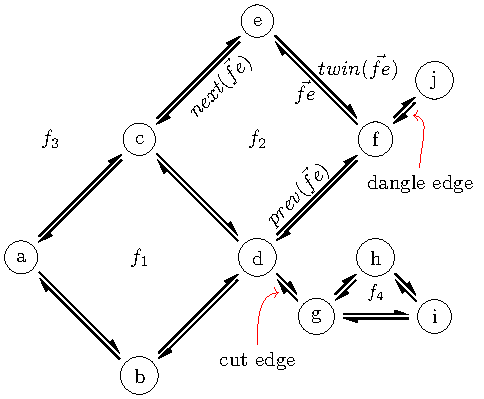
\includegraphics[width=0.6\linewidth]{chapterExtension/dcel_example2}
    \caption{Components of the DCEL structure with dangle and cut edges.}\label{fig:extension_dcel_example}
\end{figure}

The rest of this chapter is organized as follows.  Section \ref{sec:extension_methods} details the polygon extraction process for line input adaptation. It also extends the overlay method by supporting the overlay of dangle and cut edges. In Section \ref{sec:extension_experiments} we also provide additional experiments, to quantify the benefits of the kd-tree based strategy, as well as the performance on the datasets with large volumes of line segments.

\section{Related Work}\label{sec:related}
The fundamentals of the DCEL data structure were introduced in the seminal paper by Muller and Preparata  \cite{muller_finding_1978}. The advantages of DCELs are highlighted in \cite{preparata_computational_1985, berg_computational_2008}. Examples of using DCELs for diverse applications appear in \cite{barequet_dcel_1998, boltcheva_topological-based_2020, freiseisen_colored_1998}.
Our related work lies in two main areas, namely, \textit{overlay operations} and \textit{polygonization}, each discussed below.

\textbf{Overlay operations}.
Once the overlay DCEL is created by combining two layers, overlay operators like union, difference, etc., can be computed in linear time to the number of faces in their overlay \cite{freiseisen_colored_1998}. 
Currently, few sequential implementations are available: LEDA \cite{mehlhorn_leda_1995}, Holmes3D
\cite{holmes_dcel_2021} and CGAL \cite{fogel_cgal_2012}. Among them, CGAL is an open-source project widely used for computational geometry research. To the best of our knowledge, there is no scalable implementation for the computation of DCEL overlay.

While there is a lot of work on using spatial access methods to support spatial joins, intersections, unions etc. in a parallel way (using clusters, multicores or GPUs), \cite{challa_dd-rtree_2016, sabek_spatial_2017, li_scalable_2019, franklin_data_2018, magalhaes_fast_2015, puri_efficient_2013, puri_mapreduce_2013} these approaches are different in two ways: (i) after the index filtering, they need a time-consuming refine phase where the operator (union, intersection etc.) has to be applied on each pair of (typically) complex spatial objects; (ii) if the operator changes, we need to run the filter/refine phases from scratch (in contrast, the same overlay DCEL can be used to run all operators.)

\vspace{4pt}

\textbf{Polygonization}.
All available implementations for the polygonization procedure are built upon the JTS/GEOS implementation \cite{web:jts:polygonizer, web:geos:polygonizer}. 
While the JTS library is used in many modern distributed spatial analytics systems~\cite{PVK21}, including Hadoop-GIS \cite{AWV+13}, SpatialHadoop \cite{EM15}, 
GeoSpark \cite{YZS18}, and SpatialSpark \cite{YZG15}, the implementation of the polygonization algorithm \cite{web:jts:polygonizer} has not been extended to 
work in these distributed frameworks.


A data-parallel algorithm for polygonizing a collection of line segments represented by a data-parallel bucket PMR quadtree, a data-parallel $R$-tree, and a data-parallel $R^+$-tree was proposed in ~\cite{HS03}. 
The algorithm starts by partitioning the data using the given data-parallel structure (i.e., the PMR quadtree, the $R$-tree, or the $R^+$-tree), beginning the polygonization at the leaf nodes. 
The polygonization starts by finding each line segment's left and right polygon identifiers in each node. Then children nodes are merged into their direct parent node, at which redundancy is resolved. This procedure is recursively called until the root node is reached, where all line segments have their final left and right polygon identifiers assigned. 
Each merging operation partitions the input data into a smaller number of partitions. At each iteration, the number of partitions decreases while the number of line segments entering and exiting each iteration remains constant.
This implies that at the last iteration, the whole input line segment dataset must be processed on only one partition at the root node level.
In the era of big data, where the use of commodity machines as worker nodes is common, this becomes a bottleneck when processing datasets of hundreds of millions of records on one machine.
While our work and the approach in \cite{HS03} rely on iterative data re-partitioning, \cite{HS03} uses a constant input to each iteration while significantly decreasing the number of partitions.
On the other hand, our input size decreases as the number of partitions decreases (thus avoiding processing the whole dataset on a single partition).


\section{Methods}
This section explains two alternative methodologies to find moving flock patterns in large spatio-temporal datasets using modern distributed frameworks to
divide and parallelize the workload.  Before to explain the details of our contributions we will explains the in a general manner the details of the current
state-of-the-art to highlight the challenges and drawbacks at the moment to dealt with very large spatio-temporal datasets.

\subsection{The BFE algorithm}
The alternatives we will discuss later follows closely the steps explained at \cite{vieira_2009}.  In this work, the authors proposed the Basic Flock Evaluation (BFE) algorithm to find flock patterns on trajectory databases.  The details of the algorithm can be accessed at the source but we will explain the main aspects in a general view.  It is important to clarify that BFE runs in two phases: firstly, it finds valid disks in the current time instant; secondly, it combines previous flocks with the recently discovered disks to extend them and report them.  

The main inputs of the BFE algorithm are a set of points, a minimum distance $\varepsilon$ which will define the diameter of the disks where the moving entities should lay, a minimum number of entities $\mu$ at each disk and a minimum duration $\delta$ which is the minimum number of time units the entities should be keep together to be considered a flock.  Based on these inputs,  figure \ref{fig:MF_flowchart} breaks down schematically the work flow  of this phase where we can identify 4 general steps.  The main goal of this phase is to find a set of valid disks at each time instant to allow further combinations with subsequent sets of disks coming in the future.

\begin{figure}
    \centering
    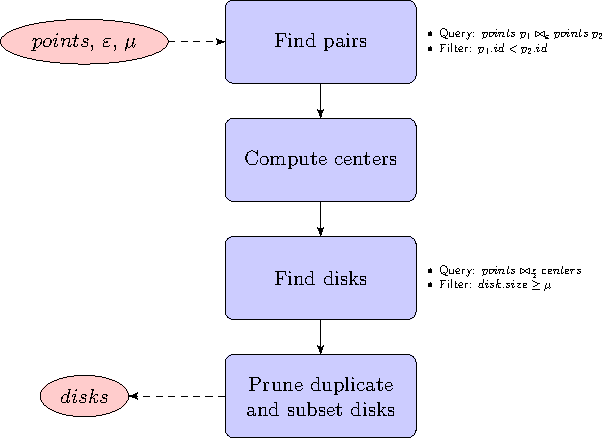
\includegraphics[width=\linewidth]{figures/MF_flowchart}
    \caption{General steps in phase 1 of the BFE algorithm.}\label{fig:MF_flowchart}
\end{figure}

The main steps in phase one can are explained as follows:
\begin{enumerate}
    \item Pair finding:  Using the $\varepsilon$ parameter, the algorithm query the set of points to get the set of pairs which laid at a maximum distance of $\varepsilon$ units.  Usually, it is a distance self-join operation over the set of points using $\varepsilon$ as the distance parameter.  The query also pays attention to do not return pair duplicates.  For instance, the pair between point $p_1$ and $p_2$ is the same that pair between $p_2$ and $p_1$ and just one of them should be reported (the id of each point is used to filter duplicates).
    \item Center computation:  From the previous set of pairs, each tuple is the input of a simple computation to locate the centers of the two circles of radius $\frac{\varepsilon}{2}$ which circumference laid on the input points.  The pseudocode of the procedure can be seen in appendix \ref{app:centers}.
    \item Disk finding: Once the centers have been identified, a query to collect the points around those centers is needed in order to group the set of points which laid $\varepsilon$ distance units each other.  This is done by running a distance join query between the set of points and the set of centers using $\frac{\varepsilon}{2}$ as the distance parameter. Therefore, a disk will be defined by its center and the IDs of the points around it. At this stage, a filter is applied to remove those disks which collect less than $\mu$ entities around it.
    \item Disk pruning: It is possible than a disk collects the same set of points, or a subset, of the set of points of another disk.  In such cases the algorithm should report just that one which contains the others.  An explanation of the procedure can be seen in appendix \ref{app:disks}.
\end{enumerate}

It is important to note that BFE also proposes a grid index structure in this phase to speed up spatial operations.  The algorithm divides the space area in a grid of $\varepsilon$ side (see figure \ref{fig:grid} from \cite{vieira_2009}).  In this way, BFE just processes each grid and its 8 neighbor grids.  It does not need to query grids outside of its neighborhood given that points in other grids are far away to affect the results.

\begin{figure}
    \centering
    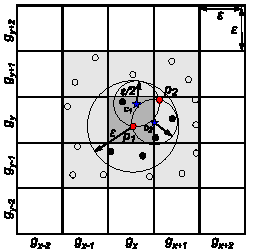
\includegraphics[width=0.4\textwidth]{figures/grid2}
    \caption{The grid-based index structure proposed at \cite{vieira_2009}.}\label{fig:grid}
\end{figure}

The second phase is more straightforward.  Figure \ref{fig:FF_flowchart} explains schematically what is done once the set of current disks (as explained in figure \ref{fig:MF_flowchart}) is found at every time instant.  This phase performs a recursion using the current set of disks and the previous set of flocks which comes from the  previous time instant.  Due to we do not know where and how far a group of entities can move in the next time instant, a cross product between both sets is required.  

\begin{figure}
    \centering
    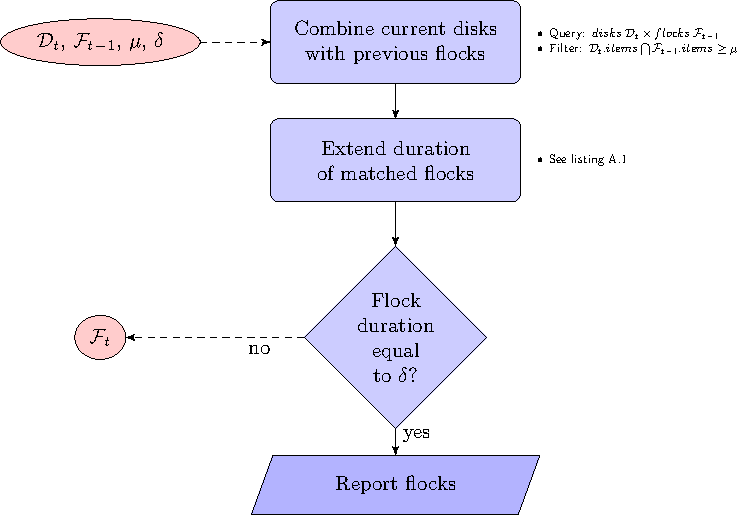
\includegraphics[width=\linewidth]{figures/FF_flowchart}
    \caption{Steps in BFE phase two. Combination, extension and reporting of flocks.}\label{fig:FF_flowchart}
\end{figure}

However, just disks which match the entities of previous flocks are kept.  Indeed, only when the size of common items is greater than $\mu$ we keep the pair.  Then, it updates the end time and duration of the filtered flocks.  This information is used to decide if it is time to report a flock or keep it for further analysis.  If the duration has reached the minimum duration $\delta$, a flock is reported and removed from the set.  The remaining flocks are sent to the next iteration for further evaluation in the next time instant.

Similarly, figure \ref{fig:FF_stages} illustrates the recursion and how the set of flocks from previous time instants feeds the next iteration.  The example assumes a $\delta$ value of 3, so it starts reporting flock since time instant $t_2$.  Note that time instants $t_0$ and $t_1$ are initial conditions.  At the very beginning of the execution, we just can find valid disks at $t_0$ which immediately are transformed to flocks of duration 1 and feed the next time instant.  At $t_1$ we can find a new set of disks $\mathcal{D}_1$ which combines with the set of previous flocks $\mathcal{F}_0$.  It updates the information of each flock accordingly but it does not report any flock yet.  From now on, subsequent time instants follows strictly the steps summarized on figure \ref{fig:FF_flowchart}.

\begin{figure}[!ht]
    \centering
    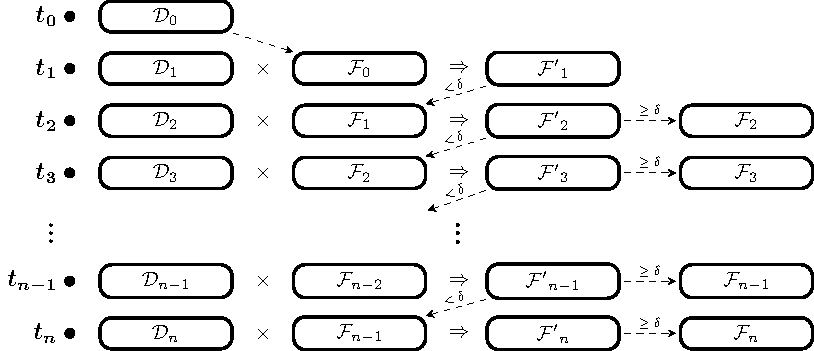
\includegraphics[width=\linewidth]{figures/FF_stages}
    \caption{BFE phase 2 example explaining the recursion of the set of flocks along time instants and the initial conditions.}\label{fig:FF_stages}
\end{figure}

\subsection{Bottlenecks in BFE and possible solutions}
There are some steps during the execution of BFE which are particularly affected when it deals with very large datasets.  Firstly, we will focus on phase 1 of BFE.  In figure \ref{fig:example}, the steps of this phase are illustrated for a sample dataset.  You can see that the number of centers and disks found is considerable large in comparison with the final set of valid disks.  Indeed, the finding of centers and the following operations grows quadratic depending on the number of points and possible pairs (which itself depend on the $\varepsilon$ parameter).   

\cite{vieira_2009} claims that the number of centers, and consequent disks, to be evaluated is equal to $2\lvert\tau\rvert^2$ where $\tau$ is the number of trajectories.  However, our experience show that there are a large number of duplicate and subset disks which are later pruned in the final stage.  This behaviour is exacerbated no just in very large datasets but also in those with areas with high density of moving entities.

\begin{figure*}
    \centering
    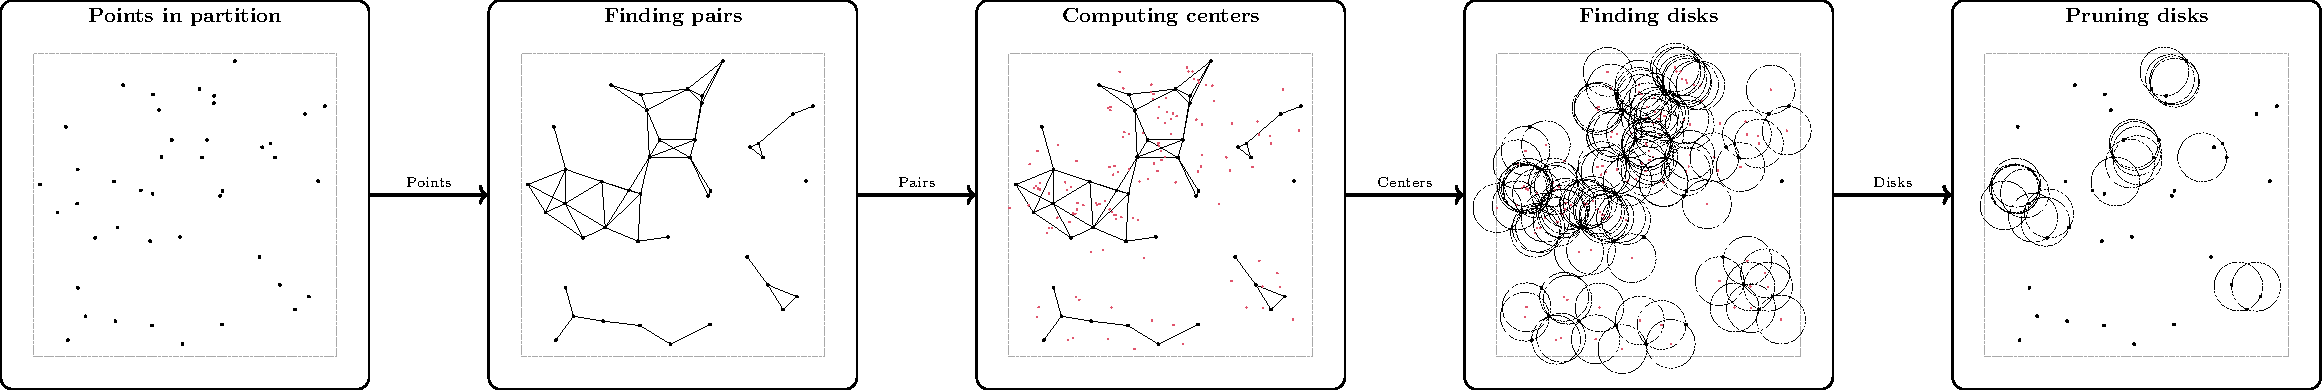
\includegraphics[width=\linewidth]{figures/MF_stages/flow}
    \caption{Example of BFE execution on a sample dataset.}\label{fig:example}
\end{figure*}

As solution for this issue, we proposed a partition strategy to divide the study area in smaller sections which can be evaluated in parallel.  The strategy has three steps: first, a partition and replication stage, then the flock discovery in each local partition and finally the merge stage where we collect and unify the results.  Let's explain each stage in more detail:

\begin{itemize}

\item Partition and Replication: Figure \ref{fig:partrep} shows a brief example of the partition and replication stage.  Note that it is possible to use different types of spatial indexes (grids, r-tree, quadtree, etc.) to create spatial partitions over the input dataset.  In the case of the example we use a quadtree which creates 7 partitions.  Now, we need to ensure that each partition has access to all the required data to complete the finding of flocks locally.  To accomplish this, all the points laying at $\varepsilon$ distance of the border of its partition are replicated to adjacent partitions.  At the right of figure \ref{fig:partrep},  it can be seen each partition surrounded by a dotted area with the points which need to be copied from its neighbor partitions.  At this point, each partition is ready to be submitted to different nodes for local processing.

\begin{figure}
    \centering
    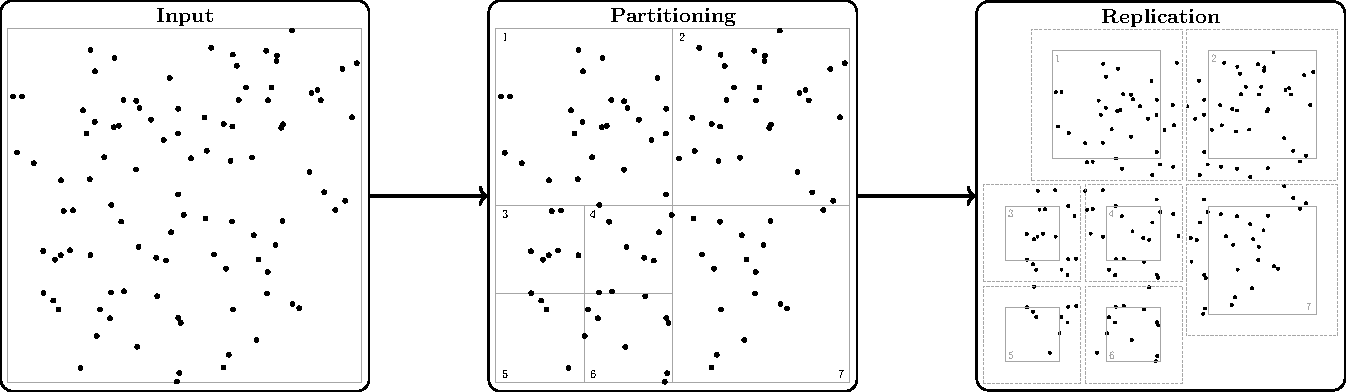
\includegraphics[width=\linewidth]{figures/MF_stages/P123}
    \caption{An example of partitioning and replication on a sample dataset.}\label{fig:partrep}
\end{figure}

\item Local discovery: Once we have all the data we need at each partition we can run the steps of the phase 1 of the BFE algorithm locally (as were explained on figure \ref{fig:MF_flowchart}).  Actually, you can see that the example of figure \ref{fig:example} describes the execution using the partition 2's points of figure \ref{fig:partrep} as sample data.

\item Merging:  In order to merge back the results we will have to pay special attention to disks laying close to the border of each partition.  We will show that if the position of disk centers lay inside of the current partition they will be safe to operate but those located in the expansion zone or outside of it will require to be treated to avoid duplicate reports.  

Disks with centers in the expansion zone will be repeated in contiguous partitions and, therefore, they will lead to duplication.  In addition, it is possible that pairs of points generates disks with centers outside of the expansion zone.  For example, Fig. \ref{fig:ensuring} illustrates the case.  Disks $a^\prime$ and $b^\prime$ are generated for points in partitions 1 and 2 respectively, however both are located outside of their expansion zone boundaries and we should to avoid to report them twice.  We present lemma \ref{lemma:disks} to show that we can safely remove those kind of disks.

\begin{lemma}\label{lemma:disks}
A disk with its center laying in the expansion zone or outside of it can be discarded as they will be correctly evaluated by one of the partitions in its neighborhood. 
\end{lemma}

\begin{proof}
  In order to support our proof we will define some concepts:  First, we will divide the area of a partition in three zones to clarify our assumptions:  we already talked about the \textit{expansion zone} as the area beyond the border of a partition (between black line and dotted red line in figure \ref{fig:ensuring}) and a width equal to $\varepsilon$.  The \textit{border zone} is a strip of width equal to $\varepsilon$ touching the interior border of a partition.  In figure \ref{fig:ensuring}, it is compromised by the dotted blue and the black lines.  The \textit{safe zone} will be the remaining internal area in the partition which is not covered by the border zone.  Second, we will call the contiguous partition which replicate a particular disk with the current one as the \textit{replicated partition}. In figure \ref{fig:ensuring}, the partition 2 is the replicated partition of partition 1 and vice versa.

  From here, it will be clear that there is a symmetric relation between the disks in the border and expansion zones in the current partition and the disks in its replicated partition.  We can certainly said that if a disk is located in the border zone of the current partition, it will be located in the expansion zone of its replicated partition.  Similarly, any disk with a center laying outside of the expansion zone of the current partition will be located in the safe zone of its replicated partition.  Keeping just the disks with centers laying in the current partition (border or safe zone) will be enough to ensure no loss of information.
\end{proof}

\begin{figure}
    \centering
    \includegraphics[width=\linewidth, page=3]{figures/merge}
    \caption{Ensuring no lost of data in safe zone and expansion area.}\label{fig:ensuring}
\end{figure}

\subsection{Additional improvements during local execution}
Even the partition strategy could reduce the size of the points to be processed at each local partition , it is possible to introduce some filter techniques which allows to reduce the impact in the creation of centers and disks and subsequent pruning.  This section explains the use of maximal cliques and minimum bounding circles (MBC) techniques as heuristics to improve the finding of disk at local level.

In graph theory, a clique is a subset of vertices forming a subgraph where all of their nodes share connections among them.  It is said that the induced subgraph is complete.  Similarly, a maximal clique happens when no additional vertex can be included in the current clique, that is, there is not a superset of vertices which could include the current clique \cite{bron_algorithm_1973}.  Although it is know that finding all maximal cliques is a problem of high complexity, studies claims that working on relatively small real-worlds graphs, they can be found in near-optimal time \cite{eppstein_listing_2010}.

Now, in our approach, it can be noted that after obtaining the set of pairs at the beginning of the BFE algorithm, we can see the result as a graph where the points are the vertices and the connections between nearby points are the edges.  So it is possible to run an algorithm (i.e. Bron-Kerbosch) over that graph to get a set of maximal cliques.

The advantage to find a set of cliques is that we will have access to set of points inside of each clique that by sure must generate one or more disks.  Given the condition of the maximal cliques, all the points inside them are $\varepsilon$ distance each other, and we can know that no other point must be included because that contradicts the definition of a maximal clique.  That constitutes a kind of sub-partitioning technique where we could do additional processing. For example, a simple filter we can apply is to remove those cliques which number of points are less than the $mu$ parameter given that those cliques will be unable to generate disks that fulfill that condition.

To introduce the next filter we need define the concept of minimum bounding circle (MBC).  Algorithms for MBC finding aims to return the center and minimum radius possible of a circle that encloses all the items of a set of points in the plane.  One of the most representative algorithm is proposed at \cite{welzl_mbc_1991} which is able to solve the problem in linear time.

The intention to use MBC algorithms at this stage is to detect maximal cliques where all their points can be enclosed in one single disk.  If that is the case, we could report directly the MBC result and save the costly computation of finding centers and pruning duplicates.  This can bring important improvements especially in datasets where the density of points is high. 

However, we have to clarify that when an unique MBC to cover all the points is not possible, the traditional steps (BFE algorithm) should be applied over them.  Finally, disks from both branches are unified and a final pruning is done to remove possible duplication.  This final step should not be costly because most of the pruning is done at maximal clique level.

Figure \ref{fig:CMBC_flowchart} shows a schematic flow chart of the steps for this alternative.

\begin{figure}
    \centering
    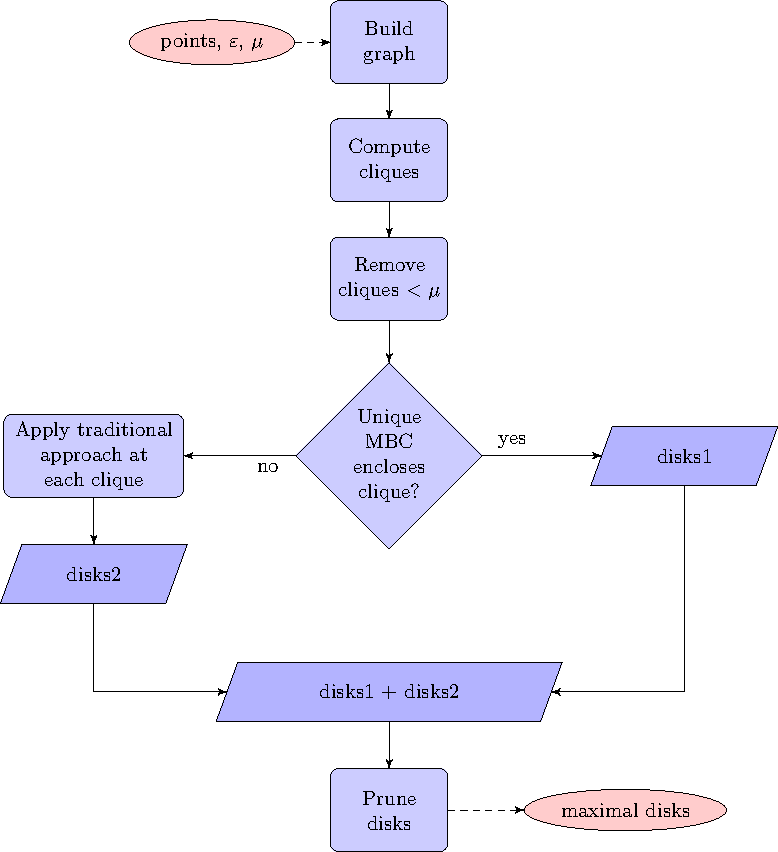
\includegraphics[width=\linewidth]{figures/CMBC_flowchart}
    \caption{Flow chart for the maximal clique and MBC filters.}\label{fig:CMBC_flowchart}
\end{figure}

\end{itemize}

\section{Scalable Polygon Extraction for Line-based Input} \label{sec:polygonization}

Our discussion so far assumed the input data is a set of clean and closed polygons in the two input layers to be overlayed. However, several real-world 
polygons, such as city blocks formed by individual road segments represented as spatial lines, are unavailable in the polygonal form. Forming polygons in such 
cases at a large scale is non-trivial and takes significant computing cost. This section further extends our scalable DCEL overlay operations to handle 
scattered line segments as input through a scalable polygonization \cite{LailaMDMPaper} process. Such a feature enables spatial data scientists to seamlessly  
exploit a rich set of publicly available datasets, e.g., spatial road networks worldwide \cite{web:data:continents,web:data:usa}.

\begin{figure}[tb]
	\centering
	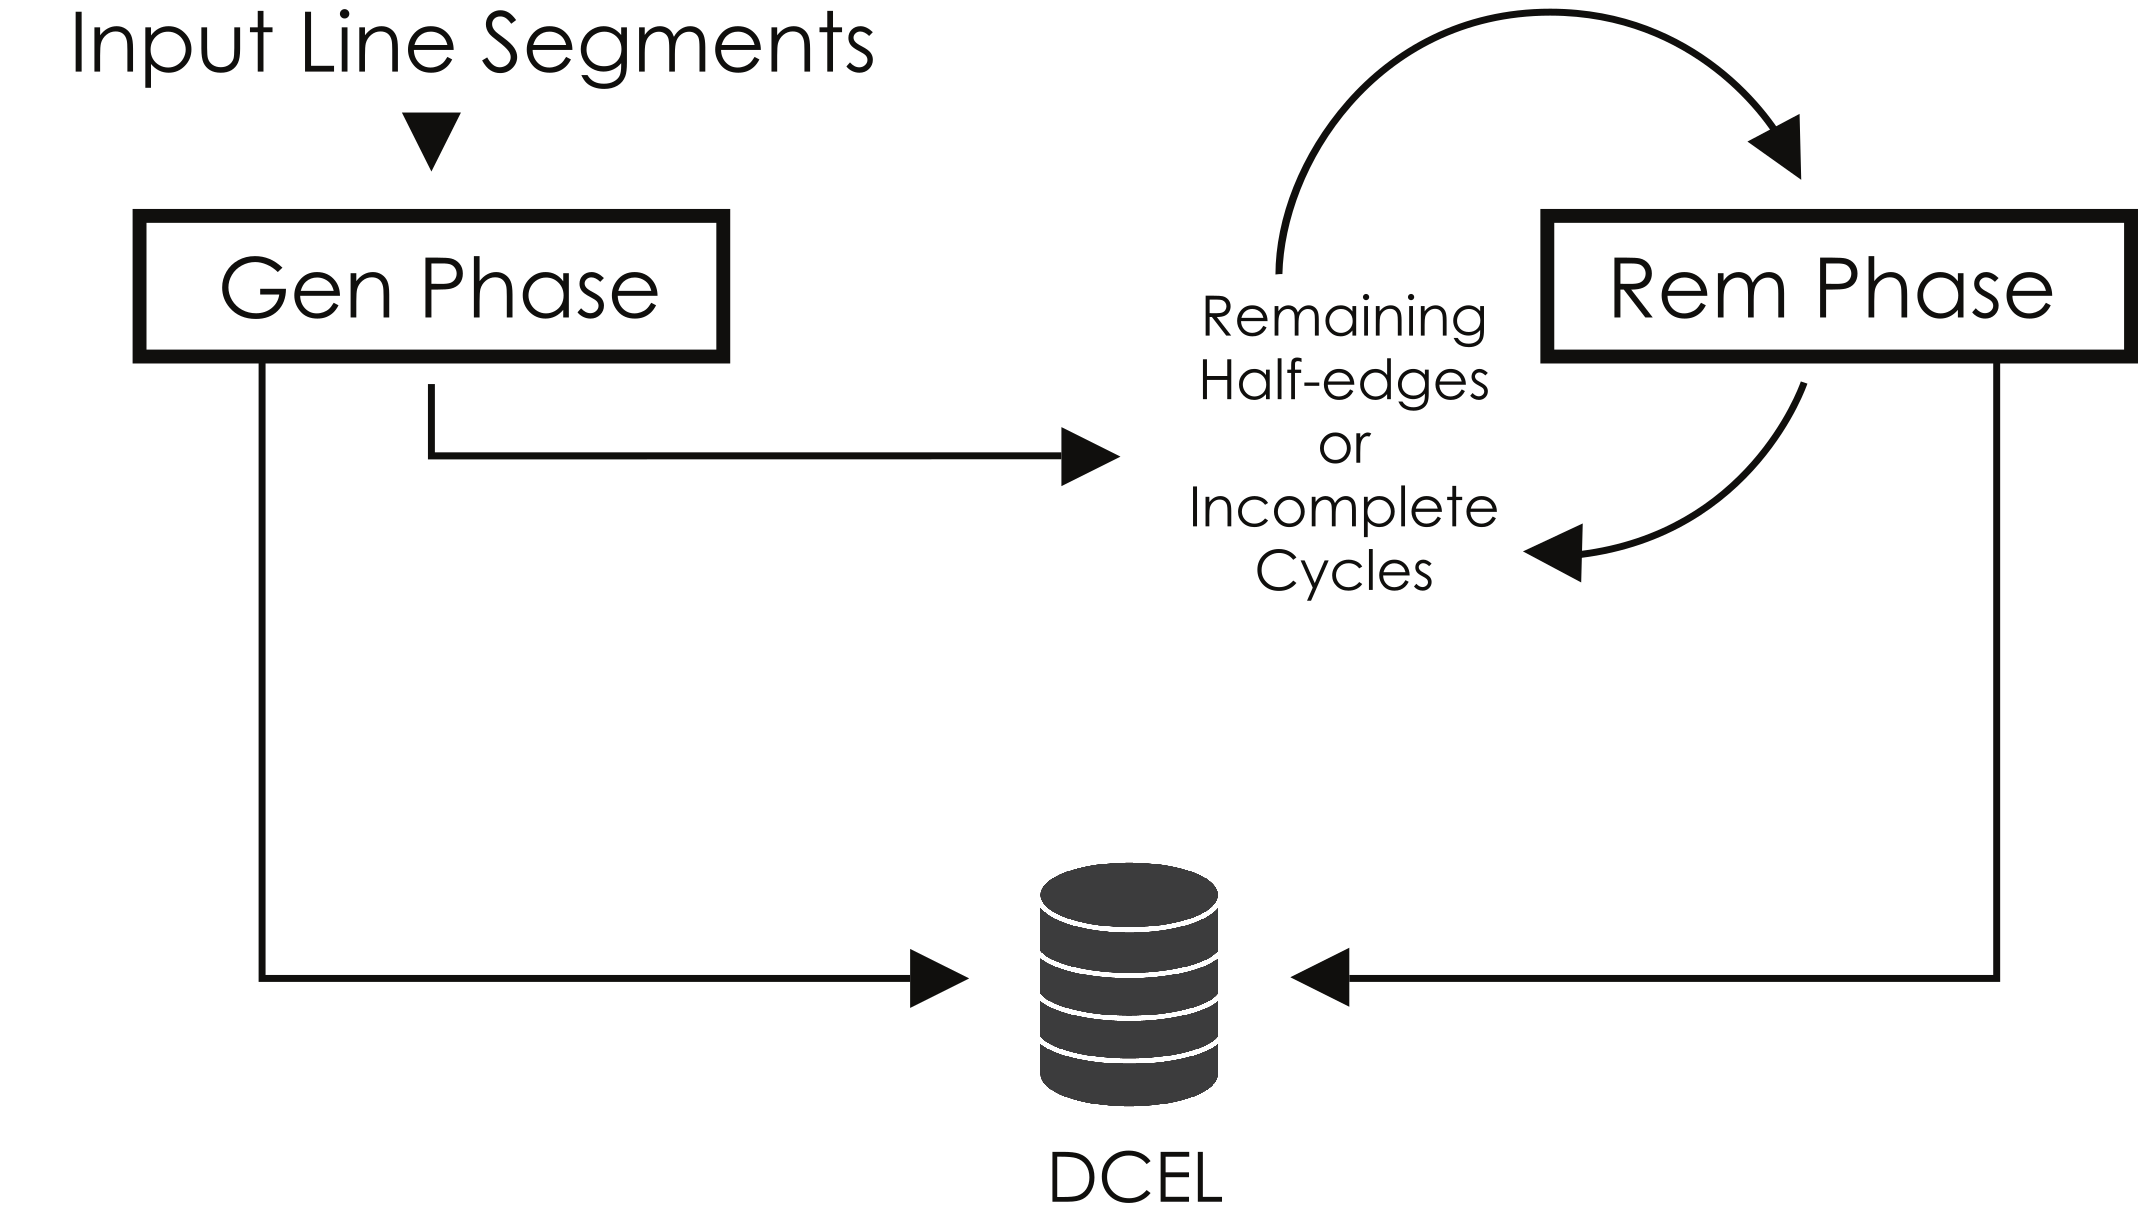
\includegraphics[width=0.75 \linewidth ]{chapter2/model/overview_updated.png}
	\caption{DCEL Constructor for Polygonization Overview}
	\label{fig:overview_ddcel}
\end{figure}

Building a DCEL data structure from an input of planar line segments extracts all closed polygons during the invocation of the \textit{polygonization} 
procedure.  In our work in \cite{LailaMDMPaper}, we proposed a scalable distributed framework to build a DCEL and extract polygons in parallel from the input 
line segments. Figure \ref{fig:overview_ddcel} shows an overview of the DCEL constructor. 

To create a DCEL data structure from input line segments, the \textit{DCEL constructor} undergoes a two-phase paradigm.  The \textit{Gen Phase}, detailed in 
Section \ref{sec:gen}, spatially partitions the input lines, generating the subdivision's vertices ($V$) and half-edges ($H$), and a subset of the 
subdivision's faces ($F_0$). 

The remaining line segments that are not assigned to a face yet are passed to the subsequent phase in the form of half-edges or incomplete cycles. An incomplete 
cycle is a connected half-edge list that is a candidate face. The \textit{Rem Phase}, detailed in Section \ref{sec:rem}, generates the subdivision's remaining 
faces, $F_j, \ \forall j > 0$. 

Section \ref{sec:partitioning_ddcel} discusses different data re-partitioning schemes with a minimal number of iterations to reduce the workload of the 
\textit{Rem Phase} without compromising correctness. The polygonization procedure produces two outputs: first, a set of closed polygons formed by the input 
planar line segments, and second, any edges that are not a part of any polygon, i.e., dangle or cut edges. Overlaying the polygons generated with any polygon 
layer follows the approaches discussed in sections \ref{sec:methods}and \ref{sec:alternative_methods}. In section \ref{sec:over_dang}, we extend the overlay 
approaches to handle overlaying a polygon layer with the remaining edges (the dangle and cut edges).

\subsection{Gen Phase}
\label{sec:gen}

The Gen phase accepts an input dataset of line segments $N$ and starts by partitioning the input across the worker nodes in a distributed cluster using a global quadtree spatial index.
Each data partition $P_i$ covers a specific spatial area represented by its minimum bounding rectangle (MBR) $B_i$.
Figure~\ref{fig:ddcel:input} shows an example of four leaf nodes of a quadtree built for input spatial line segments. Solid lines represent the line segments, and dashed lines represent the partitions' MBRs.

\begin{figure}[tb]
	\centering
	
\includegraphics[width=0.75 \linewidth ]{chapter2/model/input-network.png}
	\caption{Partitioned input spatial lines.}
	\label{fig:ddcel:input}
\end{figure}

After spatially partitioning the input lines, each partition generates its vertices, half-edges, and faces (collectively the partition DCEL) using the subset of the dataset that intersects with the partition's MBR.
The \textit{partition vertices} are the vertices that are wholly contained within the partition MBR. 
On the other hand, the \textit{partition half-edges} are any half-edge that intersects with the partition MBR.
\textit{Partition faces} are the faces that are wholly contained within the MBR of the partition.
On each data partition $P_i$, the Gen phase undergoes four main procedures; 
(1) first, generating the partition vertices and half-edges, 
(2) second, marking the dangle half-edges, 
(3) third, setting the next half-edge pointers for all half-edges and marking the cut edges, 
(4) lastly, generating the partition faces. 

\vspace{4pt}
\textit{\textbf{Step 1: Generating the Partition Vertices and Half-edges.}}
\\
In the first step, the Gen Phase starts with populating the vertices and the half-edges RDDs of the DCEL data structure.
Each partition $P_i$ receives a subset of the input dataset that intersects with the partition's boundary.
For every line segment object $o$ received at partition $P_i$ ($o \in P_i$), two vertices are generated ($v_1$, $v_2$); one for each endpoint on this line segment ($p_1$, $p_2$). These two vertices objects ($v_1, v_2$) are appended to the vertices RDD in the DCEL data structure.
We also generate two half-edges ($h_1, h_2$) for every line segment. 
The first half-edge $h_1$ has its destination vertex $v_1$, while the other half-edge $h_2$ has its destination vertex $v_2$. These two half-edges are assigned as twins.
The half-edge $h_1$ is appended to the incident list of the vertex $v_1$. Similarly, $h_2$ is appended to $v_2$'s incident list.
For a half-edge to span multiple partitions, we check whether it is wholly contained within the partition MBR $B_i$; if not, and it is just intersecting, then this half-edge spans multiple partitions. 
These half-edges are duplicated on all partitions they intersect with.
The remaining attributes of each half-edge object are assigned in the subsequent steps. 
The two generated half-edge objects ($h_1, h_2$) are appended to the half-edges RDD in the DCEL data structure.
Figure \ref{fig:ddcel:step1} shows a graphical illustration of the DCEL data structure representing the input lines after generating the vertices and the 
half-edges on all data partitions.

\begin{figure}[tb]
	\centering
	
\includegraphics[width=0.75 \linewidth ]{chapter2/model/ddcel-1.png}
	\caption{DCEL vertices and half-edges.}
	\label{fig:ddcel:step1}
\end{figure}


\vspace{4pt}
\textit{\textbf{Step 2: Marking the Dangle Half-edges.}}
\\
Dangle half-edges are not part of any face; thus, marking them is essential to exclude them during the polygonization procedure. To find dangles in the input lines, we use previously generated information, i.e., information about the vertices and their incident half-edges. 
We compute the degree of each vertex $v \in V$ populated in the previous step. A vertex degree is the number of non-dangle half-edges in its incident half-edges list. If the degree of an arbitrary vertex $v$ is less than or equal to 1 ($degree(v) \le 1$), then all of $v$'s incident half-edges and their twins are also dangle half-edges. 
Marking any new half-edge as a dangle requires recomputing the degree of the vertices connected to it. 
Thus, marking the dangle half-edges is an iterative process. After the initial run over all vertices and marking the initial dangle half-edges, we reiterate over the vertices to check for newly found dangle half-edges. We keep iterating until convergence when no new dangle half-edges are detected.


\vspace{4pt}
\textit{\textbf{Step 3: Setting the Half-edges' Next Pointers, and Marking the Cut Edges.}}
\\
The third step is divided into three smaller steps: (a) setting the next half-edge pointer for each half-edge, (b) marking the cut edges, and (c) updating the next half-edges accordingly.
To set the next pointer for each half-edge, we use information from the previous two steps, i.e., the vertices incident half-edges and the current dangle half-edges.
For each vertex $v \in V$, we sort its incident half-edges list in clockwise order, excluding the dangle half-edges. 
After sorting the incident half-edges list $v.incidentH$, for every pair of half-edges $v.incidentH[t]$, $v.incidentH[t+1]$ in the sorted list, we assign $v.incidentH[t].next$ to $v.incidentH[t+1].twin$. For the last incident half-edge in the sorted list $v.incidentH[v.incidentH.len-1]$, we assign its next half-edge to $v.incidentH[0].twin$.


After the initial assignment of the next half-edge pointers, we proceed with the second sub-step, marking the cut edges.
To mark the cut edges, we start our procedure at an arbitrary half-edge $h_{initial}$ and assign our $h_{current}$ half-edge pointer to it. We advance the $h_{current}$ pointer at each iteration to the $h_{current}$'s next ($h_{current} = h_{current}.next$), storing all visited half-edges in a list (current cycle). We keep advancing the $h_{current}$ pointer till we reach one of three cases.
(1) We return to the initial half-edge $h_{initial}$, which means a cycle is detected and no cut edge is detected.
(2) The half-edge $h_{current}.next$ is not available, which also means no cut edge is detected.
(3) We find $h_{current}.twin$ in the current cycle, which means that $h_{current}$ and its twin are both cut edges. 
Once we reach one of these cases, we mark all visited half-edges as such and proceed with a new arbitrary half-edge to be $h_{initial}$.
This process is terminated when all the partition half-edges are visited.

In the third sub-step, after marking all cut edges, we update the next pointers while excluding the cut edges. 
For each vertex $v \in V$, we sort its incident half-edges list in clockwise order again, now while excluding both the dangle and the cut edge half-edges.
After sorting the incident half-edges list $v.incidentH$, we re-execute the same process of the first sub-step, assigning $v.incidentH[t].next$ to $v.incidentH[t+1].twin$. 
Figure~\ref{fig:ddcel:step2} shows the DCEL data structure after removing the dangle and cut edges.


\begin{figure}[tb]
	\centering
	
\includegraphics[width=0.75 \linewidth ]{chapter2/model/ddcel-2.png}
	\caption{DCEL vertices and half-edges after dangle and cut edge removal.}
	\label{fig:ddcel:step2}
\end{figure}

\vspace{4pt}
\textit{\textbf{Step 4: Generating the Partition Faces.}}
\\
Polygonization on each partition $P_i$ starts with selecting an arbitrary half-edge as our initial half-edge $h_{initial}$.
We initially assign our $h_{current}$ half-edge pointer to $h_{initial}$. We advance the $h_{current}$ pointer at each iteration to the $h_{current}$'s next ($h_{current} = h_{current}.next$), storing all visited half-edges in a list $cycle$. We keep advancing the $h_{current}$ pointer till we reach one of the following cases:
(1) We return to the initial half-edge $h_{initial}$, which means that we have found a face. In this case, we add the found face $f$ to the faces collection $F_0$ and assign $h.incidentF = f, \;\; \forall h \in cycle$.
(2) The $h_{current}.next$ is not available, and $h_{current}$ is a half-edge that spans multiple partitions. In this case, the cycle needs more information from the neighboring partitions to be completed, and the current partition's data is insufficient to produce this face.
To complete this cycle, we either pass the incomplete cycle into the Rem phase (the current list $cycle$), where it collects all incomplete cycles from all partitions and attempts to join them to form a face. Another approach would be passing the plain half-edges in this cycle to the next phase. Both approaches are discussed in detail in Section~\ref{sec:rem}.
Once we finish processing this cycle, we mark all visited half-edges as such, clear the cycle, and proceed with a new arbitrary half-edge to be $h_{initial}$.
This process is terminated when all the partition half-edges are visited.
In Figure~\ref{fig:ddcel:faces}, the dotted faces are the faces generated in this phase (Gen Phase).

\begin{figure}[tb]
	\centering
	
\includegraphics[width=0.75 \linewidth ]{chapter2/model/ddcel-3.png}
	\caption{DCEL faces.}
	\label{fig:ddcel:faces}
\end{figure}

\subsection{Rem Phase}
\label{sec:rem}

The Rem Phase accepts the remaining half-edges or incomplete cycles as input. 
To be included in the remaining half-edges set, a half-edge cannot be a dangle or a cut edge. Also, the half-edge should not have been bounded to a face yet.
An incomplete cycle is a sequence of half-edges that acts as a candidate face. This incomplete cycle could not be completed since their marginal half-edges span multiple partitions.


The Rem Phase is an iterative phase, where each iteration $j$ generates a subset of faces $F_j$. The unused input data at iteration $j$ is passed to the next iteration $j+1$.
Faces generated from the Gen phase and the Rem phase constitute the whole faces of the subdivision $F$.
In each iteration, the Rem Phase starts with re-partitioning the input data across the worker nodes using a new set of partitions.
This new set of partitions satisfies the convergence criteria; the new number of partitions ($k_j$) at iteration $j$ must be less than the number of partitions ($k_{j-1}$) at iteration $j-1$. This criterion ($k_j < k_{j-1}$) ensures there is an iteration ($m$) at which the remaining line segments are re-partitioned to one partition only, where $m$ is the total number of iterations of the Rem Phase, converging the problem into a sequential one and guaranteeing the termination of the procedure.
After the data re-partitioning, we proceed with generating a subset of the remaining faces. Two approaches are employed for the remaining faces generation, depending on the phase input data.
The first approach assumes the phase input is a set of the \underline{R}emaining \underline{H}alf-edges (RH Approach). 
While the second approach assumes the input is a set of the \underline{I}ncomplete \underline{C}ycles (IC Approach). 

\vspace{4pt}
\textit{\textbf{RH Approach: Iterate over the Remaining Half-edges.}}
\\
At each iteration $j$ and on each new data partition, a subset of the remaining half-edges is received. 
Duplicate half-edges received on one new partition are merged into a single half-edge choosing the half-edge with the available next half-edge.
We follow the same procedure of generating faces in the Gen Phase. Starting from an arbitrary half-edge as our initial half-edge $h_{initial}$, we assign our $h_{current}$ half-edge pointer initially to $h_{initial}$. We advance the $h_{current}$ pointer at each iteration to the $h_{current}$'s next ($h_{current} = h_{current}.next$), storing all visited half-edges in a list $cycle$. We keep advancing the $h_{current}$ pointer till we reach one of the following cases:
(1) We return to the initial half-edge $h_{initial}$, which means that we have found a face. In this case, we add the found face $f$ to the faces collection $F_j$ and assign $h.incidentF = f, \;\; \forall h \in cycle$.
(2) The $h_{current}.next$ is not available, and $h_{current}$ is a half-edge that is not wholly contained in the new partition MBR.
Once we finish processing this cycle, we mark all visited half-edges as such, clear the cycle, and proceed with a new arbitrary half-edge to be $h_{initial}$.
This iteration is terminated when all the remaining half-edges are visited. All half-edges that have not been assigned to any face yet are passed to the next iteration.
The Rem Phase terminates if (1) there are no more remaining half-edges, i.e., all non-dangle non-cut edge half-edges are assigned to a face, or (2) the remaining half-edges have been processed on one partition.


\vspace{4pt}
\textit{\textbf{IC Approach: Iterate over the Incomplete Cycles.}}
\\
At each iteration $j$, and on each new data partition, a subset of the incomplete cycles is received. 
Starting from an arbitrary incomplete cycle $c_{initial}$ with first half-edge $first(c_{initial})$ and last half-edge $last(c_{initial})$, where the first and last half-edges are the incomplete cycle's terminal half-edges, we search for a match $c_{match}$ in the remaining incomplete cycles such that the $last(c_{initial}) = first(c_{match})$. When a match is found, we merge the two cycles such that the $last(c_{initial})$ is now the $last(c_{match})$. We keep merging cycles till we reach one of the following cases:
(1) The $last(c_{match}) = first(c_{initial})$, which means the cycle is now completed. In this case, we add the found face $f$ to the faces collection $F_j$ and remove all incomplete cycles used from the set of the incomplete cycles.
(2) We can not find a match for the current last half-edge, and the last half-edge is not wholly contained within the new partition's MBR. In this case, the incomplete cycle needs more information from the neighboring partitions to be completed, and the current partition's data is insufficient to produce this face.
Once we finish processing this matching process, we mark all visited incomplete cycles as such and proceed with a new arbitrary incomplete cycle to be $c_{initial}$.
This iteration $j$ is terminated when all the incomplete cycles are visited. All incomplete cycles that are not completed yet are passed into the next iteration.
The Rem Phase terminates if (1) there are no more remaining incomplete cycles, i.e., all cycles have been completed, or (2) the incomplete cycles have been processed on one partition.
In Figure~\ref{fig:ddcel:faces}, the hatched faces are the faces generated in the first iteration ($j=1$) of the Rem Phase.

\subsection{Data Partitioning}\label{sec:partitioning_ddcel}

The quadtree partitioner is used again to distribute the data amongst the worker nodes across the cluster. In the Gen Phase, the quadtree leaf nodes are used as the initial data partitions.
The output of the Gen Phase, whether the remaining half-edges or the incomplete cycles, is iteratively re-partitioned into new sets of partitions.
Each iteration set of partitions must satisfy the convergence criterion to ensure that the Rem Phase will terminate.
We employ the same quadtree partitioner to generate the new partitions. 
Assume we have a quadtree built on the input line segments of height $L$. 
At the Gen Phase, we use nodes at the leaf level $L$ as our initial data partitions. For each iteration $j$ in the Rem Phase, we level up in the quadtree and choose different level nodes, aside from the leaves, to be our current data partitions.  
We keep leveling up in the quadtree till we reach the root ($l=0$), which means that all data is located on only one partition (the root).
Going up in the quadtree ensures that the number of partitions at iteration $j+1$ is less than that at iteration $j$ since the number of nodes at any arbitrary level $l$ visited at iteration $j$ is more than that at level $l_{chosen}, \ \forall l_{chosen} < l$ visited at iteration $j+1$.


We always start with the leaf nodes level $L$ in the Gen Phase. Choosing which levels to visit next in each iteration $j$ is a system parameter. 
We offer different schemes for the visited quadtree levels: 
\begin{enumerate}
    \item Going directly to the root node at $l=0$ after the leaf nodes, i.e., visiting only levels L in the Gen and 0 in the Rem phases. However, the experimental evaluation shows that collecting the data after the Gen phase on one node is prohibitive, and one worker node will not be able to process the Gen phase's output.
    \item Going \underline{1} \underline{L}evel \underline{U}p (1LU) each iteration, i.e. if we visit level $l$ at iteration $j$, we go to level $l-1$ at iteration $j+1$. This means the Rem Phase visits all the quadtree levels resulting in $L$ iterations.
    \item Going \underline{2} \underline{L}evels \underline{U}p (2LU) each iteration resulting in half the number of iterations $\frac{L}{2}$ compared to 1LU.
    \item Skipping to the \underline{M}iddle of the tree at level $\frac{L}{2}$, then continue going 1 level up for the remaining levels (M1LU), which will also result in $\frac{L}{2}$ iterations.
    \item Skipping to the \underline{M}iddle of the tree every time, dividing the current level by two each iteration (MU); this will result in $\log_2(L)$ iterations.
\end{enumerate}
The goal is to find a re-partitioning scheme with a minimal number of iterations, thus reducing the workload of the Rem Phase while ensuring that the worker nodes can process the chunk of the data it receives at each iteration $j$.
The extreme case of having only one iteration at the Rem Phase will not work since the data is too big to fit one partition and be processed by only one worker node. On the other hand, the more unnecessary iterations we have, the more overhead on the system resulting in higher query latency.


\subsection{Overlaying Polygons with Dangle and Cut Edges} \label{sec:over_dang}

\begin{figure}[tb]
	\centering
	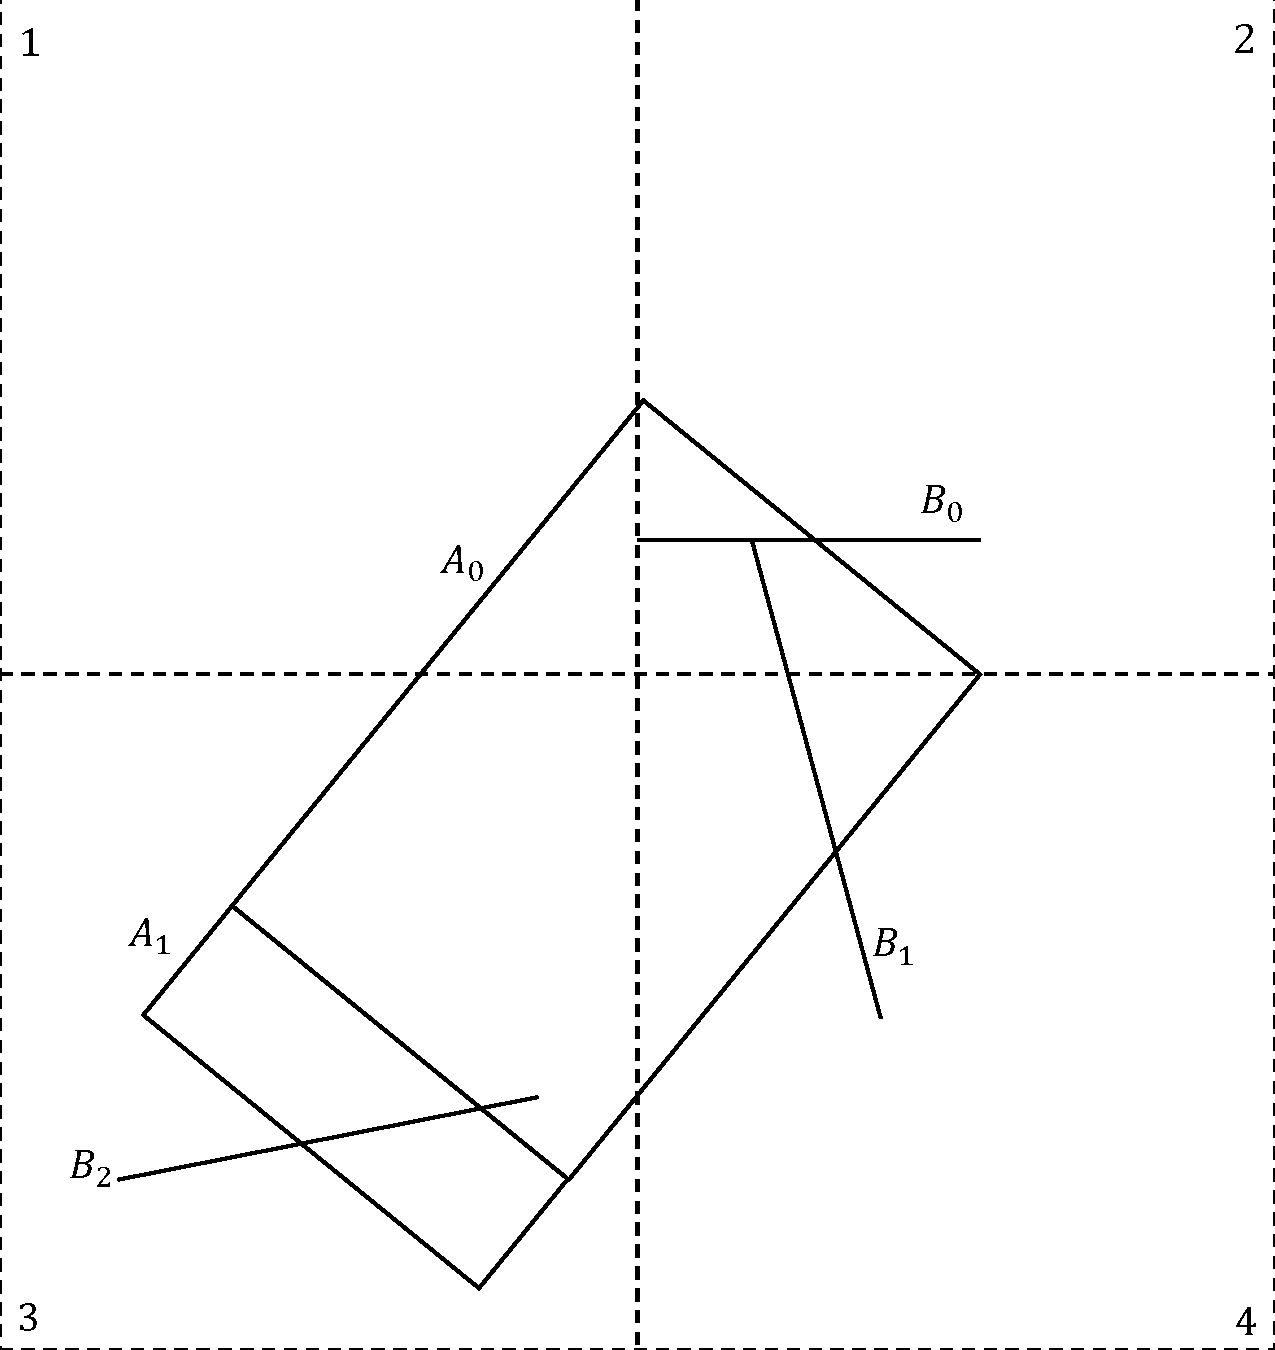
\includegraphics[width=0.75 \linewidth ]{chapter2/model/DangleOverlay1.pdf}
	\caption{Spatial partitioning of input layers A and B}
	\label{fig:dangleoverlay:input}
\end{figure}

\begin{figure}[tb]
	\centering
	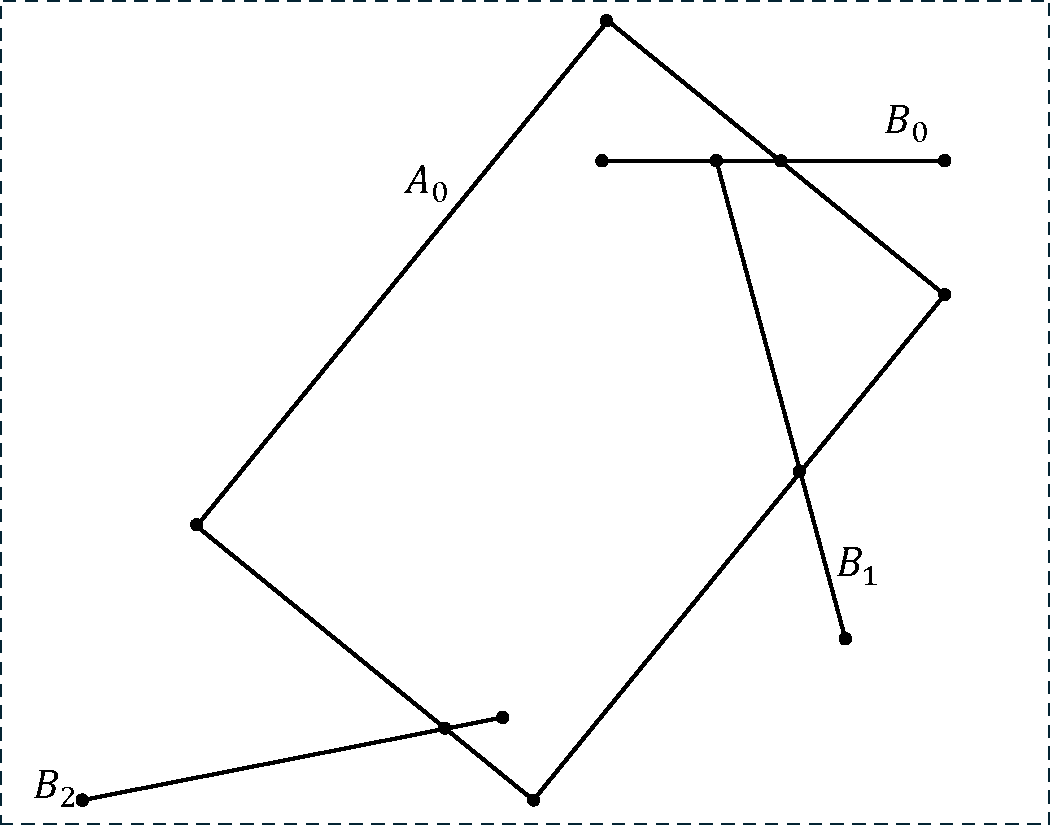
\includegraphics[width=0.75 \linewidth ]{chapter2/model/DangleOverlay2.pdf}
	\caption{Re-Partitioning of polygon $A_0$ with edges it intersects with}
	\label{fig:dangleoverlay:inter}
\end{figure}

\begin{figure}[tb]
	\centering
	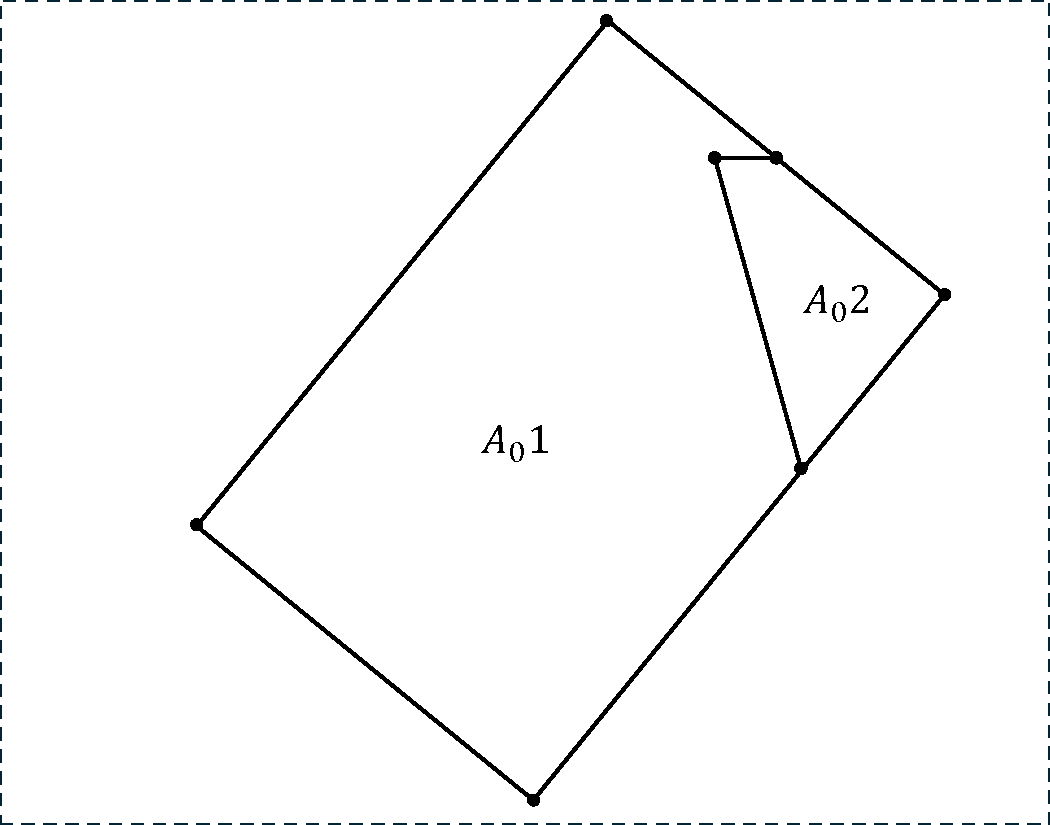
\includegraphics[width=0.75 \linewidth ]{chapter2/model/DangleOverlay3.pdf}
	\caption{The result of polygonization of $A_0$ with $B_0, B_1, B_2$}
	\label{fig:dangleoverlay:result}
\end{figure}

The polygonization procedure produces two outputs: first, a set of closed polygons formed by the input planar line segments, and second, any edges that are not 
a part of any polygon, i.e., dangle or cut edges. 
Overlaying the polygons generated with any polygon layer follows the approaches discussed in sections \ref{sec:methods} and \ref{sec:alternative_methods}.
However, we need to modify the algorithms provided in these previous sections to overlay an input polygon layer $A$ with the dangle and cut edges, i.e. layer 
$B$. In particular, we modify the reduce phase.
Figure \ref{fig:dangleoverlay:input} illustrates the spatial partitioning of the two input layers, $A$ and $B$. Layer $A$ contains two input polygons, $A_0$ and 
$A_1$, while Layer $B$ consists of three dangle edges, $B_0$, $B_1$, and $B_2$.

Each edge from layer $B$ is labeled a unique label and is fed as an input to the overlay module.
The local overlay is performed by finding intersections between the input polygon layer $A$ and layer $B$ on each data partition.
If a polygon with $id = i$ from polygon layer $A$ intersects with edges with ids $id = a, id = b, id = c$ from layer $B$ at some data partition, we generate a 
label to match these intersections $A_{i} B_{a} B_{b} B_{c}$. 
At the reduce phase, we re-partition the data by the first label, meaning we collect all edges that intersect with the first label.
If two data partitions produced the labels $A_{i} B_{a} B_{b} B_{c}$ and $A_{i} B_{x} B_{y}$, we repartition the data such that $A_{i}$ is on one partition with 
all edges it is intersecting, i.e., $B_{a}, B_{b}, B_{c}, B_{x}, B_{y}$.
In Figure \ref{fig:dangleoverlay:inter}, Polygon $A_0$ is re-partitioned along with the edges it intersects, specifically $B_0$, $B_1$, and $B_2$.

After re-partitioning the data, we have all edges from both layers intersecting each other on the same partition. The next step is to find the polygons 
generated by these intersections. Since there is no guarantee that only one polygon is generated, we substitute the polygon concatenation proposed in 
Section~\ref{sec:reduce} by performing \textit{polygonization} on each partition. The polygonization procedure ensures it generates all new possible polygons. 
The polygonization procedure follows the algorithm mentioned in Section~\ref{sec:gen}. It starts with generating the new vertices and half-edges, then marking 
the current dangles and cut edges, then setting the next pointers and finally generating the partition polygons.
Figure \ref{fig:dangleoverlay:result} shows the result of polygonizing the edges from Polygon $A_0$ and $B_0$, $B_1$, and $B_2$, resulting in two polygons, 
$A_01$ and $A_02$.

Polygons from all partitions generate the overlay between the polygon layer $A$ and layer $B$.

\section{Experimental Evaluation}
\subsection{Experimental Setup}
For our experiments, we used a cluster with 12 nodes running Linux O.S. (kernel 3.10) and Apache Spark 2.4. Each node has 8 cores (i.e. 96 cores in total), each core with an Intel Xeon CPU at 1.70GHz and 4GB of main memory.
To evaluate the various approaches, we used 3 synthetic datasets, with different characteristics as described in table \ref{tab:datasets}. To create these datasets we used the SUMO simulator \cite{SUMO2012} and imported the traffic networks of Berlin and Los Angeles from OpenStreetMap \cite{haklay2008openstreetmap}. We used the SUMO setting for pedestrians, and created 10K, 25K and 50K pedestrian trajectories. We set the total duration to 10, 30 and 60 min respectively. The generator reported the positions of these moving pedestrians every minute.

\begin{table}
    \centering
    \begin{tabular}{cccc}
        \hline
        Dataset & Number of Trajectories & Total number of points & Maximum Duration (min) \\
        \hline
         Berlin10K &  10000 & 97526 & 10\\ 
         LA25K &  25000 & 1495637 & 30\\
         LA50K &  50000 & 2993517 & 60\\
         \hline
    \end{tabular}
    \caption{Datasets}
    \label{tab:datasets}
\end{table}

For the partitioning phase we used a quadtree structure (other indices can be used as well; the advantage of the quadtree is that it tries to create nodes with similar number of objects). 
Our input is a set of points \textit{(traj-id, x,y,t)}. To build the quadtree, we sample 1\% of the input and insert this subset of points to an empty quadtree. For a quadtree, the user needs to set a parameter for the node capacity $c$. When the number of points that fall in a node overpass $c$ the node splits. After all sample points are inserted, we use the Minimum Bounding Rectangles (MBRs) of the leaves as the partitions of our approach. All the remaining points are then inserted in these fixed partitions (i.e., no more splitting occurs). Each partition will be assigned to a different cluster node which will run a sequential version of BFE or PSI, run locally on the points of that partition.

\subsection{Optimal number of partitions for phase 1.}
Clearly the capacity parameter $c$ directly affects the number of partitions. A low value of $c$ leads to a large number of partitions. This in return will generate many smaller jobs to be distributed over the cluster. However, the cost of transmission and possibly replication increases, which could become a bottleneck.  On the other hand, large $c$ implies a smaller number of partitions, which will create larger individual jobs, increasing the time response required by the sequential algorithm in each partition. 

Figure \ref{fig:optimal_performance} shows the execution time (in seconds) for finding the maximal disks (phase 1) for a given time instant, under different values of $c$ and for various values of $\varepsilon$. The LA25K dataset was used for these experiments. 
Consider the case $\varepsilon = 20m$; clearly there is a value of $c$ that minimizes the time to find the maximal disks ($c=100$, which corresponds to around 1300 partitions). 
It can also be seen that the optimal value for $c$ varies depending on $\varepsilon$.  For example, for smaller $\varepsilon = 2m$, the execution time is minimized for a larger capacity  $c=500$ (which corresponds to around 250 partitions).
When $\varepsilon$ is large, there will be larger number of pairs and thus maximal disks to compute. Using a smaller $c$ creates more partitions (for the same spatial area) thus reducing the amount of work per partition.

\begin{figure}
    \centering
    \begin{tabular}{c c}
         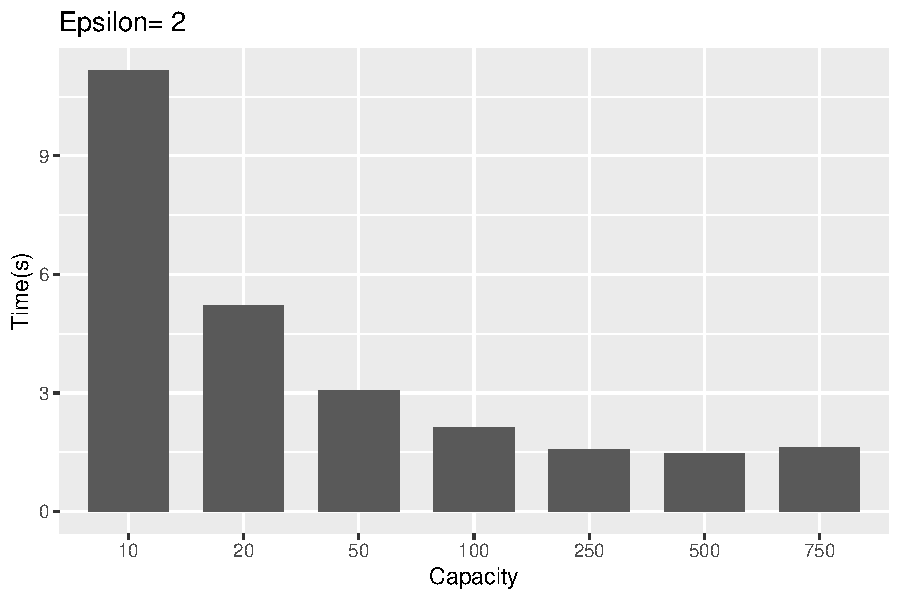
\includegraphics[width=0.45\linewidth]{figures/plots/01_optimal_performance/pflockE2_by_capacity.pdf} & 
         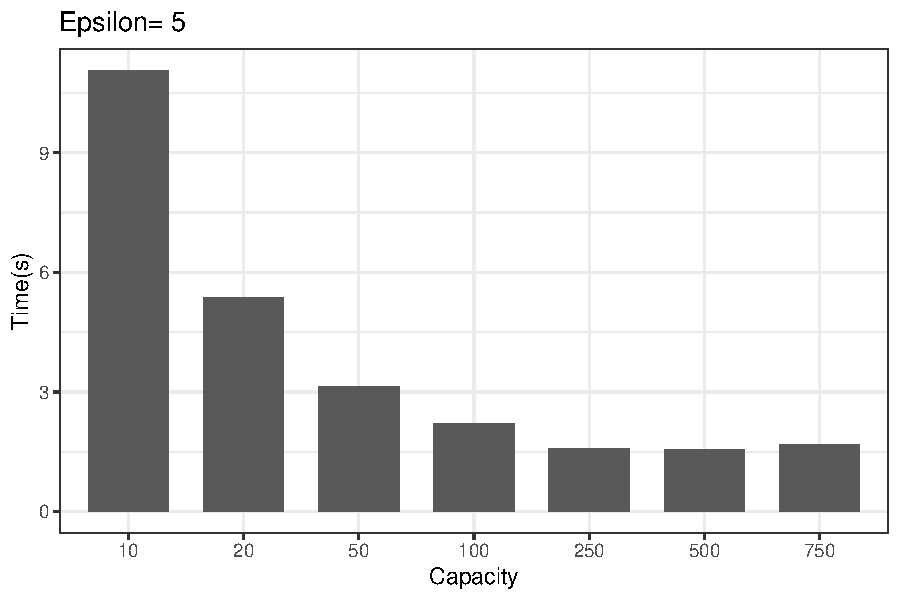
\includegraphics[width=0.45\linewidth]{figures/plots/01_optimal_performance/pflockE5_by_capacity.pdf} \\
         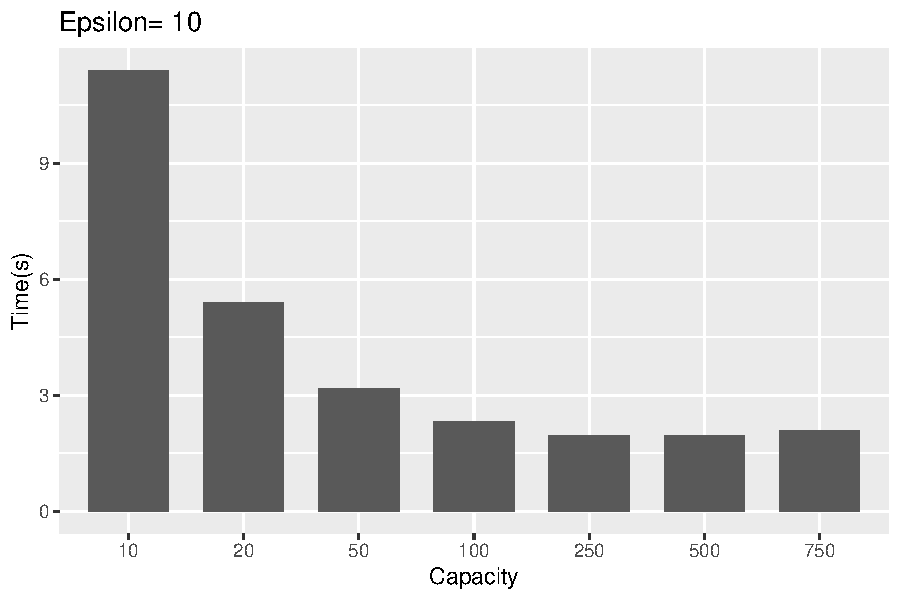
\includegraphics[width=0.45\linewidth]{figures/plots/01_optimal_performance/pflockE10_by_capacity.pdf} &
         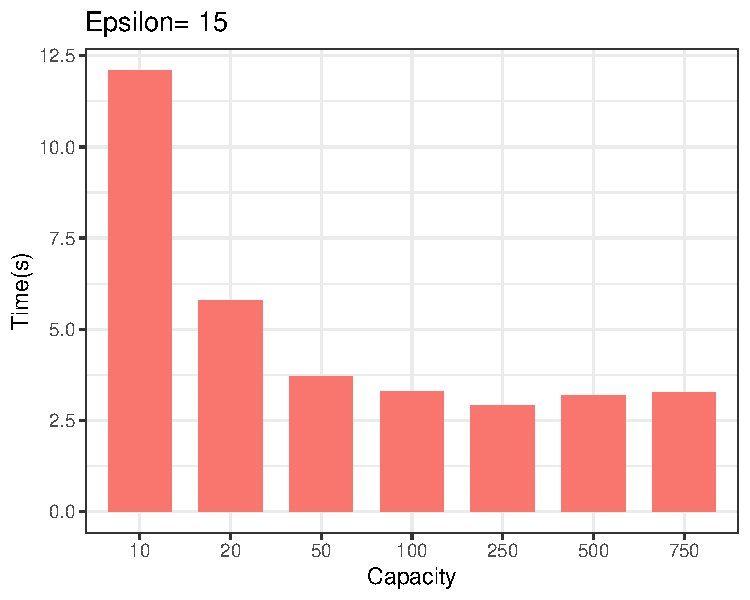
\includegraphics[width=0.45\linewidth]{figures/plots/01_optimal_performance/pflockE15_by_capacity.pdf} \\ 
         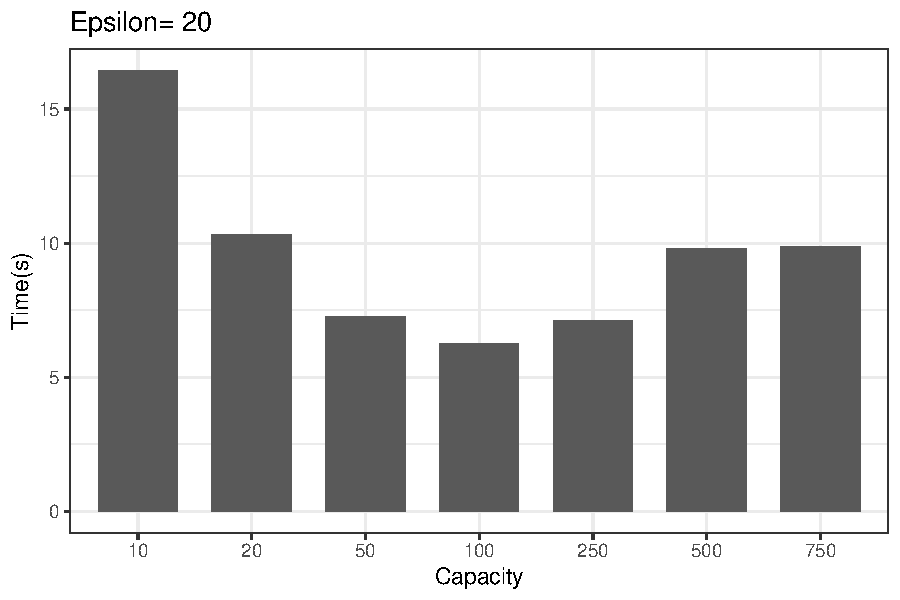
\includegraphics[width=0.45\linewidth]{figures/plots/01_optimal_performance/pflockE20_by_capacity.pdf} & \\
    \end{tabular}
    \caption{Execution time testing different values for Capacity ($c$) and Epsilon  $\varepsilon$).}\label{fig:optimal_performance}
\end{figure}

Having set the optimal value of $c$ for a given $\varepsilon$ value, we further explored the behavior of BFE and PSI for the most `demanding' partitions, that is, those partitions that took the most time to compute phase 1. Since partitions run in parallel on different cores, these are the partitions that will affect the overall performance.  

\subsection{Analyzing most costly partitions.}
We first identified the top-10 partitions that take most time to run the BFE algorithm with $\varepsilon$ = 20 meters. For these specific partitions we run both BFE and PSI while varying $\varepsilon$ from 10 to 20 meters. Figure \ref{fig:top_time_partitions} 
shows the phase 1 execution times; we see that the PSI performance was consistently better than BFE. 

\begin{figure}
    \centering
    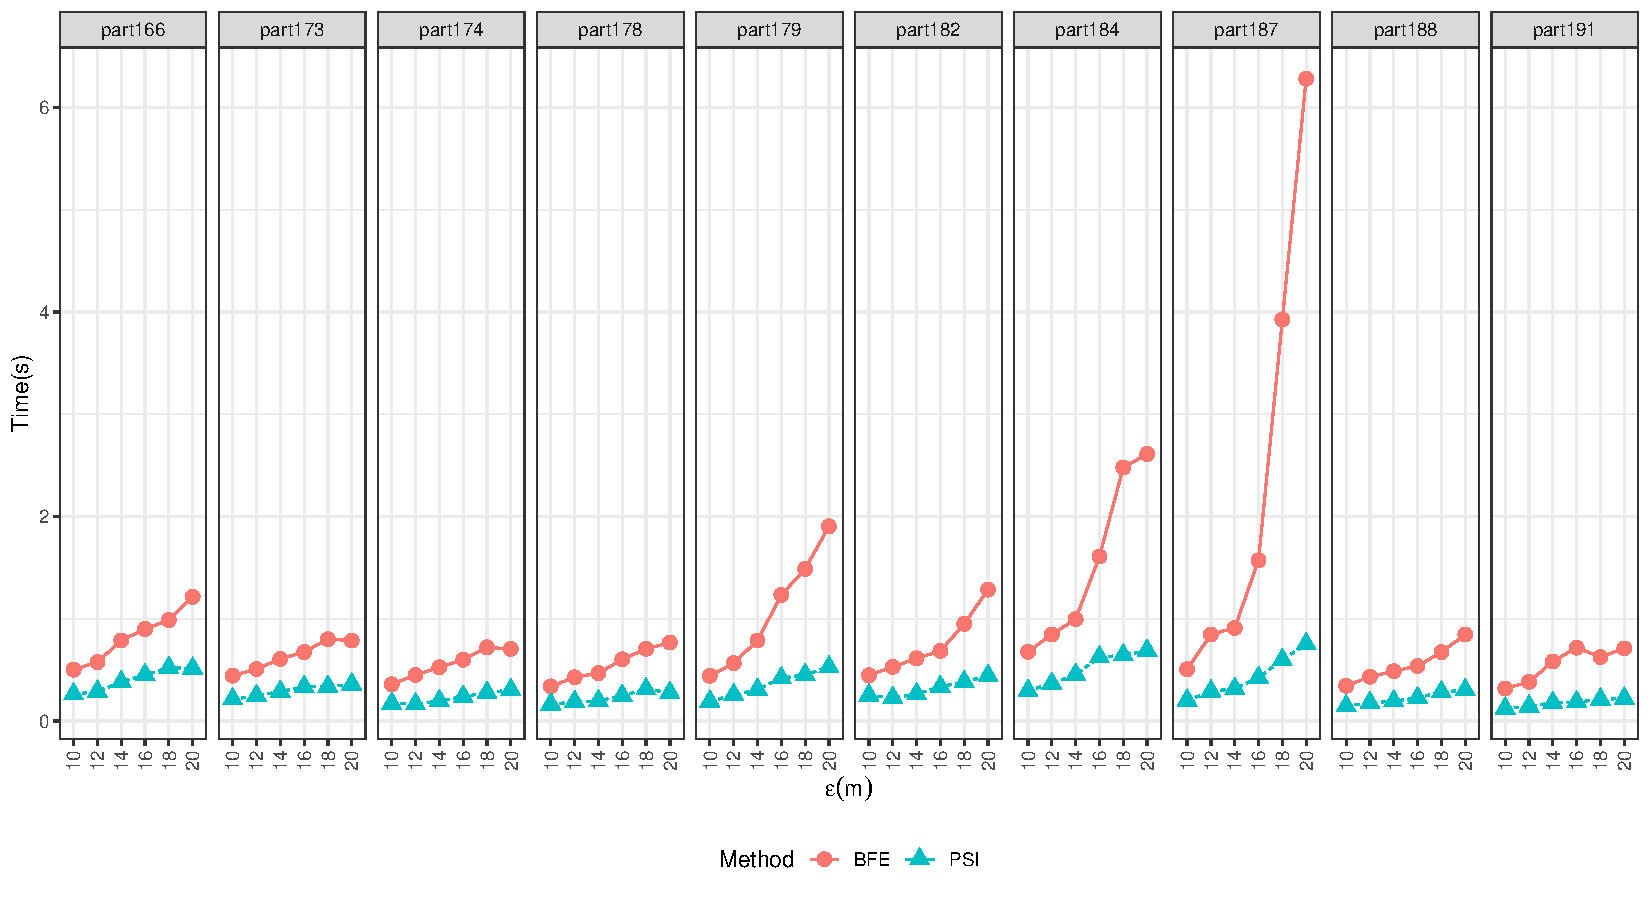
\includegraphics[width=\linewidth]{figures/plots/03_top_time_partitions/top_time_partitions.pdf}
    \caption{Comparing the performance of PSI and BFE for time consuming  partitions.}\label{fig:top_time_partitions}
\end{figure}

We further examined what causes some partitions to take more time than others. Figure \ref{fig:pairs_performance} shows the phase 1 execution times per partition while varying $\varepsilon$ from 10m to 20m. Partitions are ordered by the number of pairs they contain. A first observation is that we $\varepsilon$  increases, the number of pairs also increase since higher $\varepsilon$  allows for more maximal disks. For example, for $\varepsilon$=10m the highest number of pairs in a partition is around 1800. In contrast, for $\varepsilon$ =20m, there are partitions with almost 4000 pairs. Another observation is that BFE is more affected than PSI by the density of pairs in a partition. This is depicted more clearly for $\varepsilon$ =18m or 20m. As mentioned earlier, the flexible boxes that PSI uses (see Figure \ref{fig:square}) better identify the points needed for computing the pairs; instead BFE uses a fixed grid cell. 

A final observation is that there are few partitions that take much more time than others, those that are more dense with pairs (as this relates to the number of disks that have to be computed and later pruned). For example, the partition that takes more time for $\varepsilon$ =20m in the Figure, is the one with most pairs (which shows as partition 187 in Figure \ref{fig:top_time_partitions}). 

We thus further examine how the processing for phase 1 is divided in the most `demanding' partition. Figure \ref{fig:dense_stages}.a (.b) shows the processing taken by each of the phase 1 stages (see Figure \ref{fig:example}) of BFE (respectively PSI) for partition 187. 
It can be seen that the most expensive stage is the final procedure of filtering the disks whose points are included in other disks, that is identifying the `Maximal' disks (shown as Maximals in the figure). This is because both BFE and PSI need to scan a large set of candidate disks looking for those which could contain others and remove the rest. It is clear that this processing increases as $\varepsilon$ increases, since the number of pairs and subsequent candidates disks also increases with $\varepsilon$.

\begin{figure}
    \centering
    \begin{tabular}{c c}
        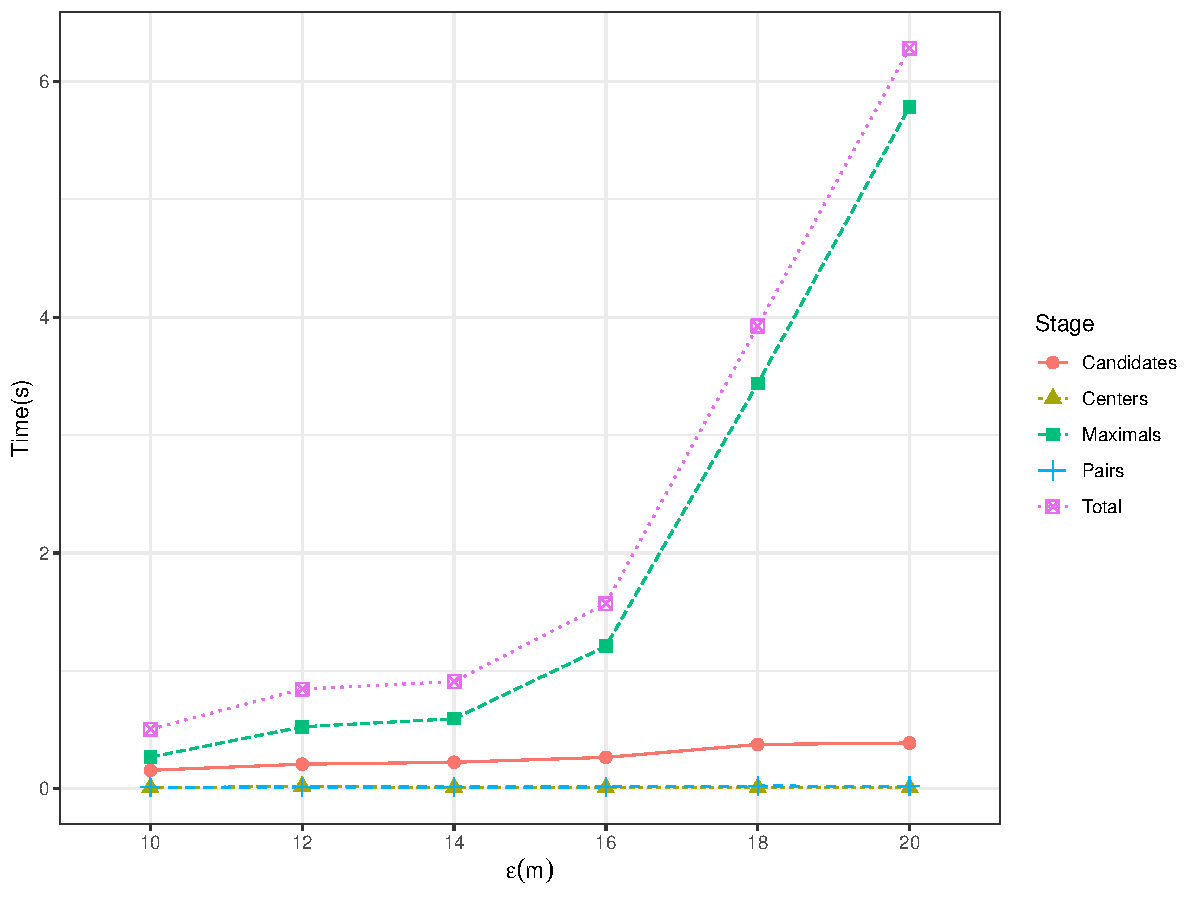
\includegraphics[width=0.49\linewidth] {figures/plots/09_dense_stages/dense_stages_bfe.pdf} &
        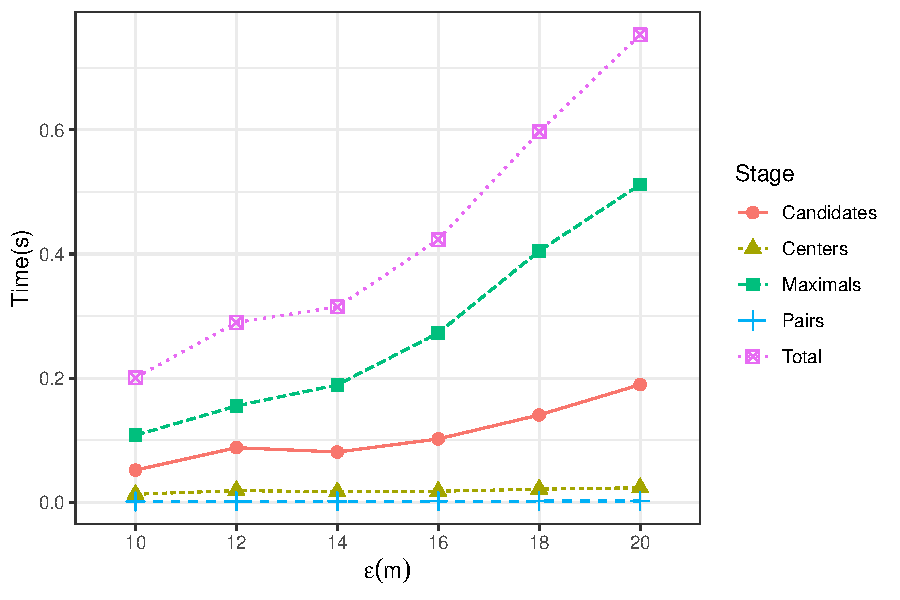
\includegraphics[width=0.49\linewidth] {figures/plots/09_dense_stages/dense_stages_psi.pdf} \\
        (a) & (b) \\
    \end{tabular}
    \caption{Processing time for the stages of Phase 1, in (a) BFE, (b) PSI.}\label{fig:dense_stages}
\end{figure}

\begin{figure}
    \centering
    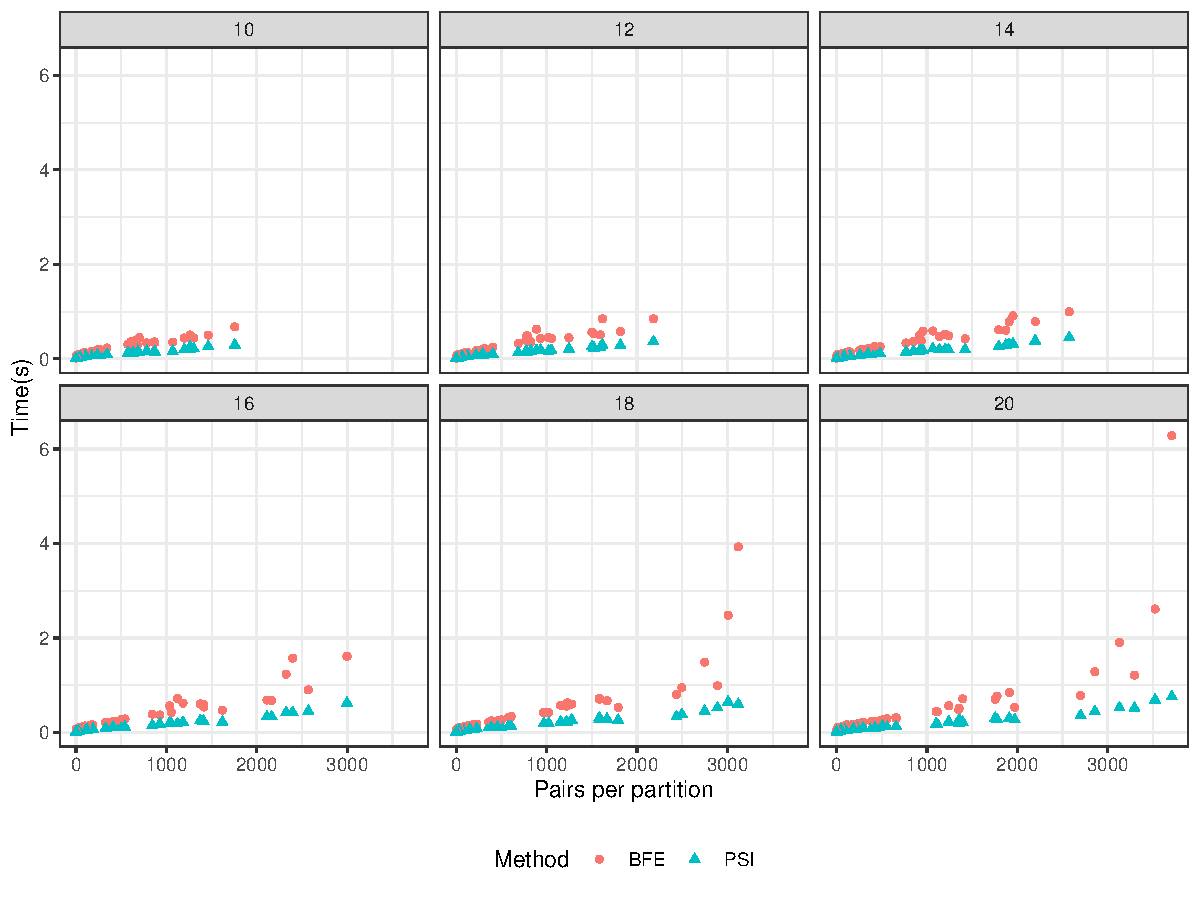
\includegraphics[width=0.85\linewidth]{figures/plots/04_pairs_performance/pairs_performance.pdf}
    \caption{Execution time for pairs/disks finding in the dense partition.}\label{fig:pairs_performance}
\end{figure}

\subsection{Can we reduce pruning time?}
Dense areas are problematic for pruning as they are very sensitive to an increase in the value of $\varepsilon$, creating an enormous number of pairs. Therefore, we explored ideas that may lead to more effective grouping of points. It should be noted that density based spatial clustering approaches (e.g. DBSCAN \cite{dbscan}) will not work since very dense areas will result in one large cluster, thus not solving the issue. Moreover, clustering does not enforce strong relationship among all elements in the cluster (which is something we need for a flock: all points are within $\varepsilon$ from each other).

Instead, we explored graph-oriented clustering, and in particular the notion of \textit{maximal cliques}. In an undirected graph, a maximal clique is a subset of vertices where each vertex is directly connected to every other vertex in the subset; further the subset is maximal in the sense that it cannot be further extended by adding a new vertex \cite{tomita_clique_2013, bron_algorithm_1973}. 
One could consider the points in a partition as the vertices of an undirected graph and add edges that connect those pairs of points that are within $\varepsilon$ distance. 
Finding the set of maximal cliques in this graph will provide subsets of points which are directly connected to ALL the other members in the subset, that is, all points in the subset are at most $\varepsilon$ apart from each other and no other point could be added to the subset. 
However, not all maximal cliques are maximal disks. 
A maximal clique is a maximal disk if it has at least $\mu$ points and can be enclosed by a disk with radius $\frac{\varepsilon}{2}$.

To check this condition, we introduce the concept of Minimum Bounding Circle (MBC) \cite{welzl_mbc_1991}. Given a set of points in the Euclidean space, a MBC is the smallest circle that contains all the points. For each maximal clique found in a partition, we could quickly check if the points in this clique are all inside a MBC with diameter $\varepsilon$. If this is the case, we can directly report that set of points and their MBC as a maximal disk. However those cliques that not fulfill the restriction must be evaluated in the traditional way (i.e., for the clique points we must compute centers, find disks, prune disks as in Figure \ref{fig:MF_flowchart}).

To evaluate the cliques that do not pass the above condition, we used two variants. The first one (termed COLLECT) collects the points from \textit{all} the cliques that are not reported as maxima disks, removes duplicates (points that appear in many cliques) and apply the traditional method of pruning for the whole set. In the second (noted as EACH) we apply the pruning procedure over the points of each such clique independently. Figure \ref{fig:cmbc_variants} shows the performance of the variants compared with the time employed by BFE for the same stage (a) and the PSI (b).  It turns out that the performance of the variants does not improve the execution time. Looking more closely at each approach we can observe that while finding the cliques (and their MBCs) does not take much time, nor many of these cliques are maximal disks. The overhead to find the maximal disks from the remaining cliques is large, making the original approach faster for both the BFE and PSI.

\begin{figure}
    \centering
    \begin{tabular}{c c}
        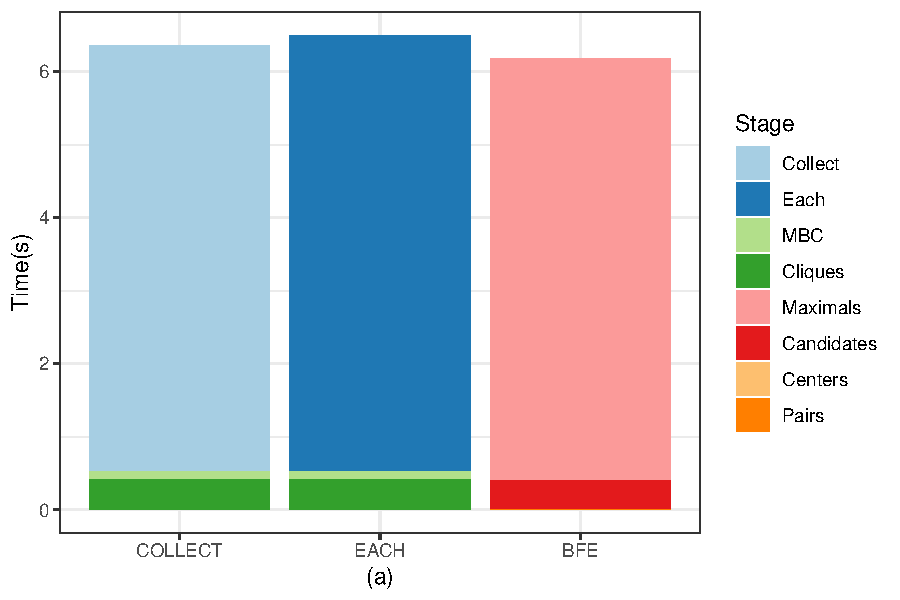
\includegraphics[width=0.49\linewidth] {figures/plots/10_cmbc_variants/cmbc_bfe.pdf} &
        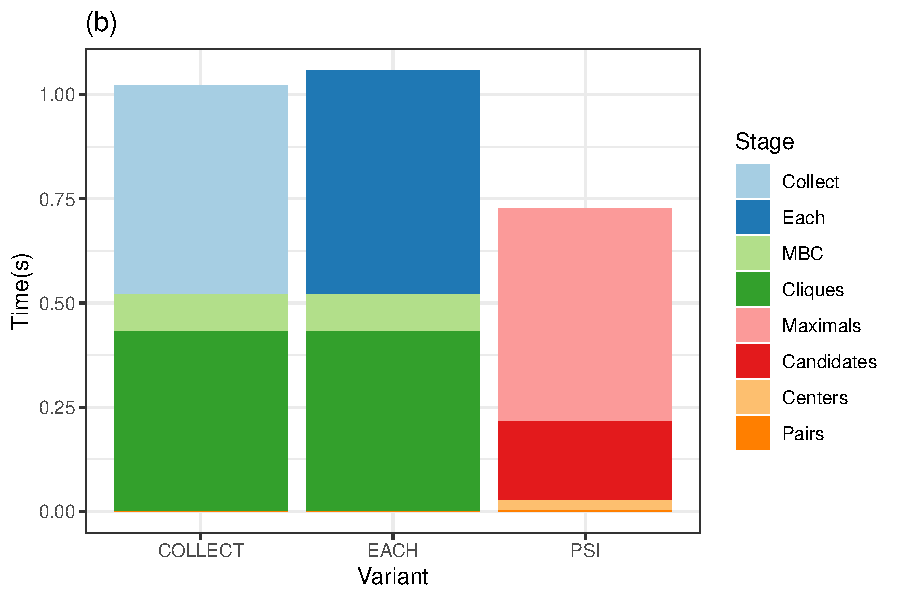
\includegraphics[width=0.49\linewidth] {figures/plots/10_cmbc_variants/cmbc_psi.pdf} \\
        (a) & (b) \\
    \end{tabular}
    \caption{Execution time of the Cliques approach compared to (a) standard BFE and (b) standard PSI.}\label{fig:cmbc_variants}
\end{figure}

\subsection{Uniform dataset.}
To better examine the relative behavior of the scalable BFE and PSI approaches, we also considered a synthetic dataset where we could control the values of $c$, $\varepsilon$ and the point density. We used a fixed square area of 1000m x 1000m and placed 25K, 50K, 75K and 100K points uniformly distributed in this area. 
We used various quadtree capacities ($c$ equal to 100, 200 and 300) that gave us different number of partitions (see Table ~\ref{tab:uniform_ncells}). We run both BFE and PSI for finding the maximal disks of phase 1, using different $\varepsilon$ values (from 1m to 5m). The results appear in Figure \ref{fig:uniform_performance}. While we again see that overall PSI has better performance than BFE, there are cases (for small $\varepsilon$ values) where BFE is better. In those cases, the small $\varepsilon$ creates fewer pairs and the ordering that PSI requires is an overhead. Nevertheless, in the remaining experiments where we consider the temporal joins (phase 2, flock creation) we concentrate on the scalable performance of PSI. 

\begin{table}
    \centering
    \begin{tabular}{c|cccc}
              & 25K & 50K  & 75K  & 100K \\
        \hline
        c=100 & 544 & 1024 & 1024 & 2185 \\
        c=200 & 256 & 514  & 1024 & 1024 \\
        c=300 & 256 & 514  & 481  & 1024 \\
    \end{tabular}
    \caption{Number of partitions by capacity and number of points in uniform datasets.}
    \label{tab:uniform_ncells}
\end{table}

\begin{figure}
    \centering
    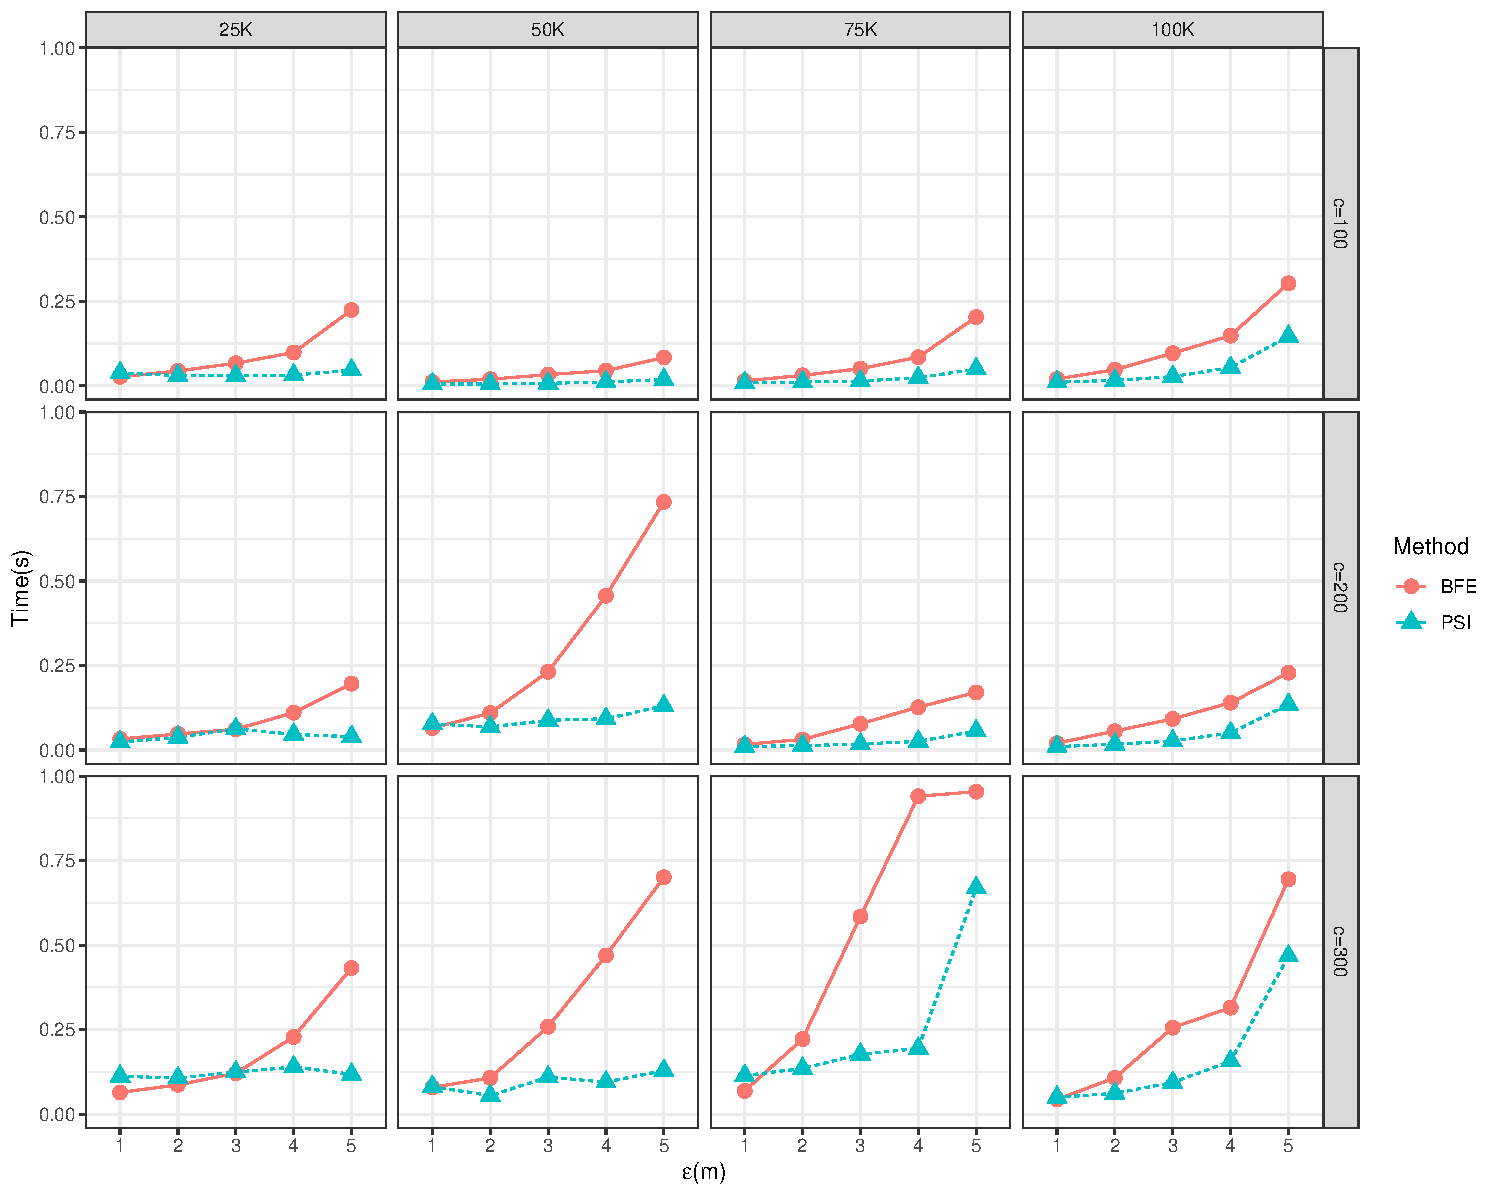
\includegraphics[width=\linewidth]{figures/plots/05_uniform_performance/uniform_performance.pdf}
    \caption{Performance in an uniform dataset analysing density and capacity with diverse values for epsilon.}\label{fig:uniform_performance}
\end{figure}

\subsection{Evaluation of Phase 2: Temporal join.}
Phase 2 deals with the joining of maximal disks between time instants to create the flocks. In Section \ref{sec:temporal_join} we discussed four alternatives: Master, Level, LCA and Cube-based. For these experiments we use the scalable PSI approach given its robust performance. First we compared the Master and By-Level alternatives for varying $\varepsilon$ from 20 to 40m using the Berlin10K dataset (see Figure \ref{fig:step_performance}). For By-Level we examined different options for the Step (from 1 to 6). The Master approach is the slowest given the overhead of sending all the CPFs to the root node. The By-Level approach performance depends on the Step. Small step (i.e. step 1) adds the overhead that CPFs may need to be evaluated in more intermediate nodes until completed. A larger Step value reduces parallelism as more CPFs are send to intermediate nodes. Based on these experiments we set Step=3.

We also evaluated the best value for the \textit{interval} parameter for the Cube-based approach. We tested different values for the interval parameter using the LA25K dataset with $\varepsilon=30m$. This dataset has a total of 30 time instants, and we varied the interval parameter from 2 to 12 time instants.  The results appear in Figure \ref{fig:interval_performance}. Lower interval values imply higher parallelism (more cubes that can be processed independently) but we need to check more cube crossings for CPFs which adds to the execution time. On the other hand, large intervals, reduce parallelism but also reduce the number of CPF crossings. Based on these results, we set $interval=6$ for the Cube-based approach.   

\begin{figure}
    \centering
    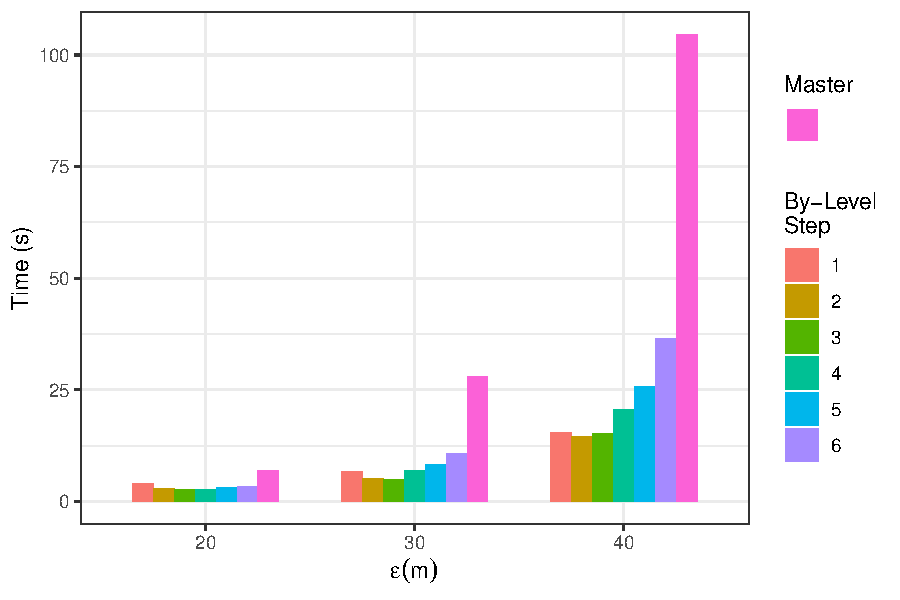
\includegraphics[width=0.8\linewidth]{figures/plots/06_step_performance/step_performance.pdf}
    \caption{Root and step alternative for temporal join using the Berlin dataset (step=7 is root).}\label{fig:step_performance}
\end{figure}

\begin{figure}
    \centering
    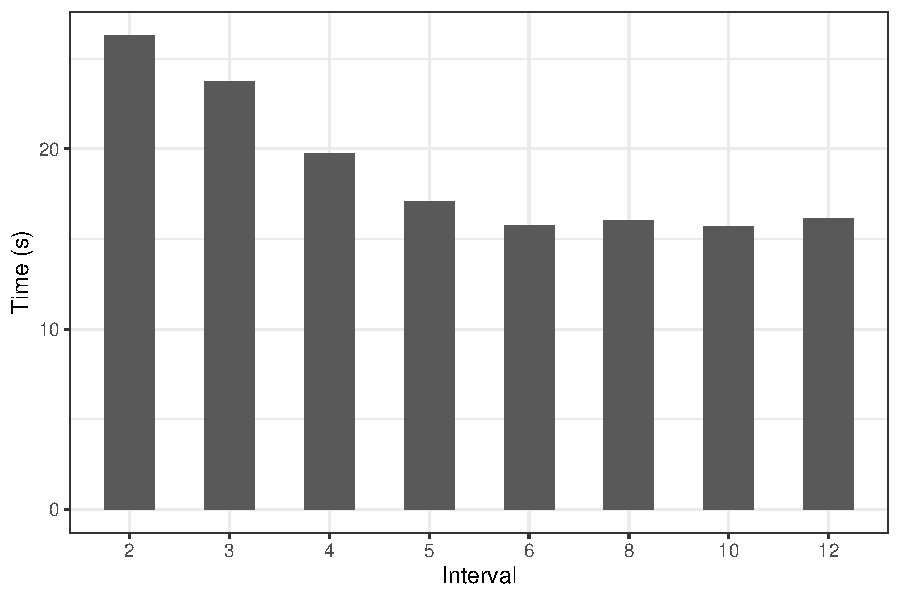
\includegraphics[width=0.8\linewidth]{figures/plots/07_interval_performance/interval-performance.pdf}
    \caption{Interval analysis for the Cube-based alternative for temporal join using the LA25K dataset.}\label{fig:interval_performance}
\end{figure}

Finally we compared the above optimized versions of By-Level and Cube-based with Master and LCA. Figure \ref{fig:la25k_e_bfe_psi} shows the results, including the sequential PSI algorithm for reference. This experiment used the LA25K dataset while varying the value of $\varepsilon$ from 5 to 30m. Clearly, all parallel approaches offer large improvement. To further analyse the relative performance of the scalable approaches, Figure \ref{fig:la25k_e} focuses on their performance for the same experiment. Interestingly, for very small $\varepsilon$ the Master approach is the best (simply because there are not many flocks, so sending the CPFs to one node is fast). As $\varepsilon$ increases, the Cube-based approach is the winner as it takes more advantage of parallelism. At the same scenario, By-Level improves over Master for the reasons explained in Figure \ref{fig:step_performance}). Similarly, for larger $\varepsilon$ LCA is faster than By-Level because it finds faster the node that can complete the CPFs.
We run the same experiment using the LA50K dataset while varying the value of $\varepsilon$ from 4 to 20m. The results appear in Figure \ref{fig:la50k_e}. Again, the Cube-based approach has the best performance as $\varepsilon$ increases.

\begin{figure}
    \centering
    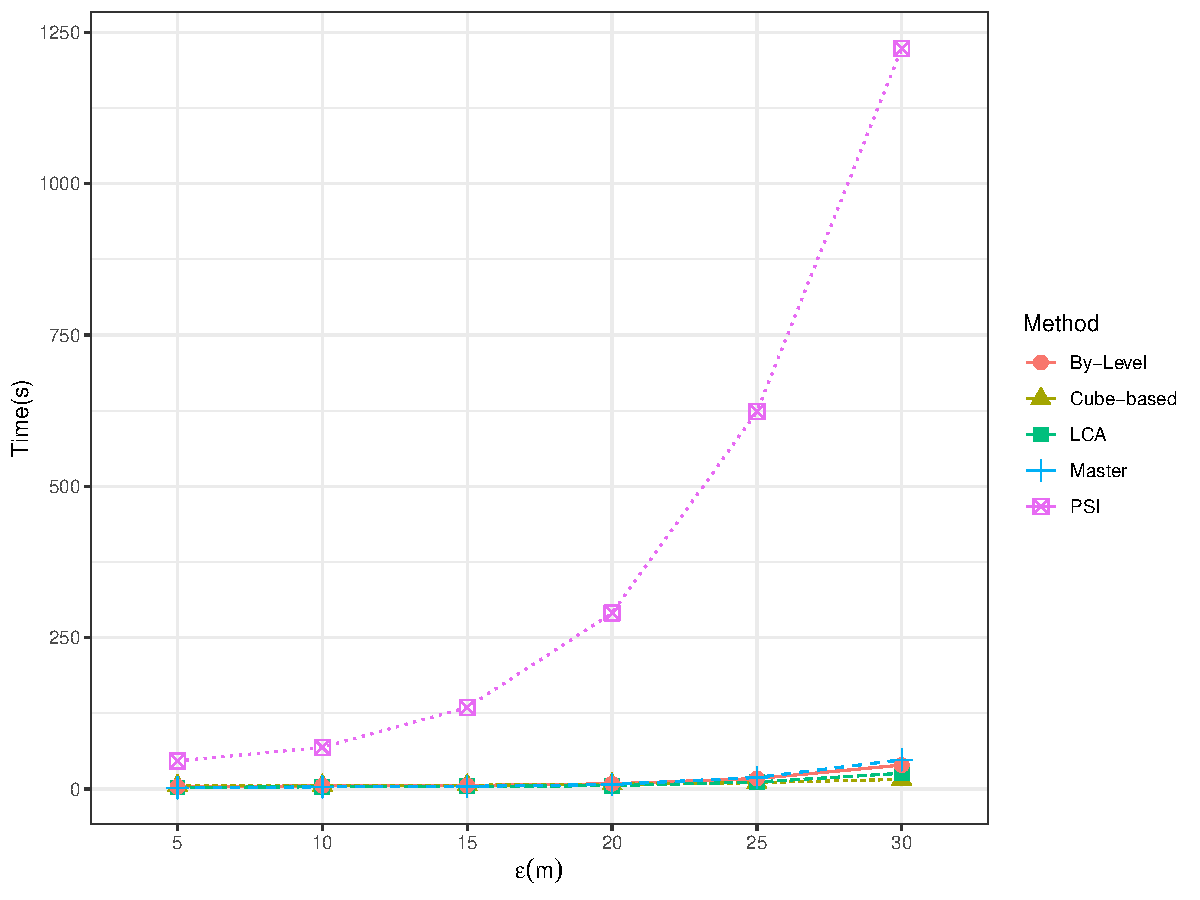
\includegraphics[width=0.75\linewidth]{figures/plots/08_sequential_parallel/la25k_e_bfe_psi.pdf}
    \caption{Performance comparing parallel and sequential alternatives in the LA25K dataset.}\label{fig:la25k_e_bfe_psi}
\end{figure}

\begin{figure}
    \centering
    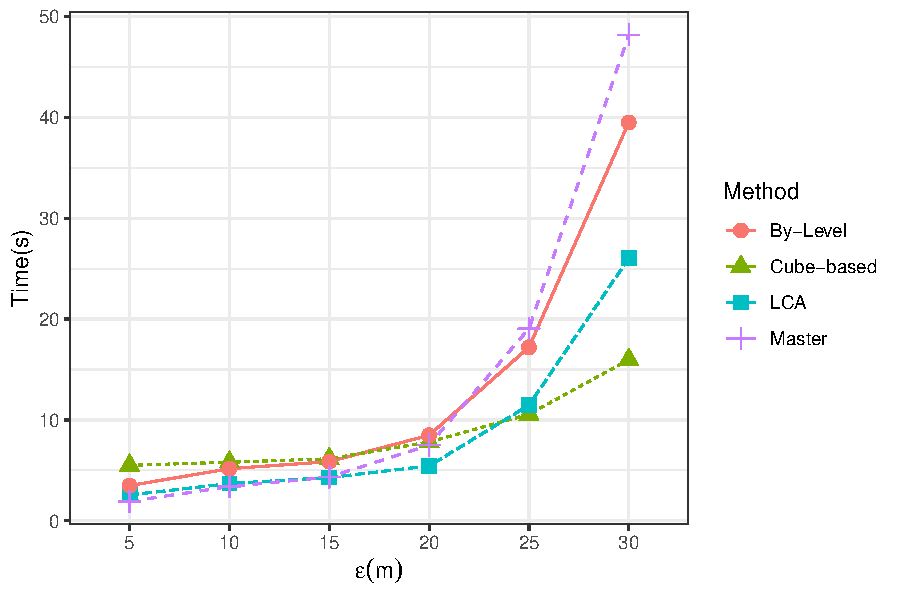
\includegraphics[width=0.75\linewidth]{chapter4/figures/plots/08_sequential_parallel/la25k_e}
    \caption{Performance of the 4 parallel alternatives in the LA25K dataset.}\label{fig:la25k_e}
\end{figure}

\begin{figure}
    \centering
    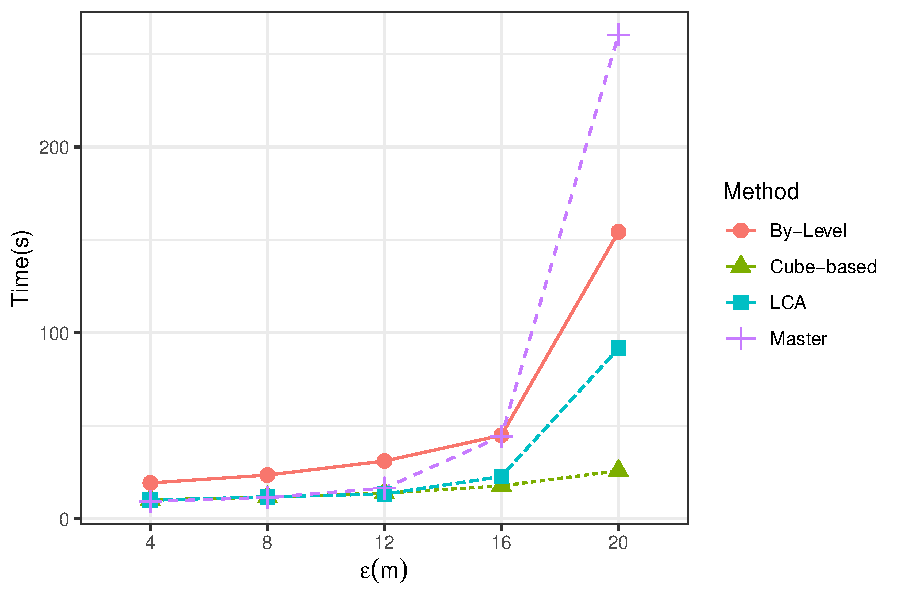
\includegraphics[width=0.75\linewidth]{chapter4/figures/plots/08_sequential_parallel/la50k_e}
    \caption{Performance of the 4 parallel alternatives in the LA50K dataset.}\label{fig:la50k_e}
\end{figure}

\section{Conclusions} \label{sec:conclusions}
We introduced SDCEL, a scalable approach to compute the overlay operation among two layers that represent polygons from a planar subdivision of a surface. Both input layers use the DCEL edge-list data structure to store their polygons. We support input polygons in clean polygon format and polygons represented by scattered line segments through scalable polygonization. Existing sequential DCEL overlay implementations fail for large datasets. We first presented two partition strategies that guarantee that each partition collects the required data from each layer to work independently. We also proposed several optimizations to improve performance. Our experimental evaluation using real datasets shows that SDCEL has very good scale-up and speed-up performance and can compute the overlay over very large layers (up to 37M edges) in a few seconds.

\backmatter

\bmhead{Acknowledgements}
We would like to thank Sergio Rey from the Center for Geospatial Sciences for introducing us to the Scalable DCEL problem.

\section*{Declarations}

\begin{itemize}
\item Funding: This work was partially supported by the National Science Foundation under grants IIS-1901379, IIS-2237348, CNS-2031418, SES-1831615 and the Google-CAHSI research grant. 
\item Data availability: Data description and access is described in the experimental section.  The sources of the dataset are publicly available and the references and cited accordingly.
\end{itemize}


%%===========================================================================================%%
%% If you are submitting to one of the Nature Portfolio journals, using the eJP submission   %%
%% system, please include the references within the manuscript file itself. You may do this  %%
%% by copying the reference list from your .bbl file, paste it into the main manuscript .tex %%
%% file, and delete the associated \verb+\bibliography+ commands.                            %%
%%===========================================================================================%%

\bibliography{sdcel,ddcel-references}% common bib file
%% if required, the content of .bbl file can be included here once bbl is generated
%%\input sn-article.bbl

\end{document}
